\section{Case study: networks trained to output a constant}\label{sec:nets}

This section tests the framework on the case that motivates it: a ReLU network
trained to always output $1$ on uniformly random inputs $x\in\{-1,+1\}^d$, and the rare
inputs on which it fails. The answer is sharply divided.
\begin{itemize}
\item \emph{Sound lower bounds work very well wherever $p$ could be checked.}
Fixed-level splitting (\cref{thm:splitting}) combined with a betting confidence bound
(\cref{prop:betting}) certifies $L/p$ of \nnSuiteRatioL{} on the exact suite (for
$p\ge10^{-5}$), and \nnScaleRatioChecked{} of a reference value $p_{\rm ref}$ on the
\nnScaleChecked{} nets at $d=32$--$128$ whose reference was checked independently
(exactly at $d=32$, by Monte Carlo down to $p\approx\nnMcBlocksMin$), with no
assumption on mixing (\cref{sec:nets-lower,sec:nets-smc}). On \nnScaleUnchecked{}
more nets, with $p_{\rm ref}$ down to \nnBigPref, it reaches \nnScaleRatioUnchecked{}
of $p_{\rm ref}$; there $p_{\rm ref}$ is the mean of more replicates of the same
estimator, which cannot reveal a failure mode that the chains never reach
(\cref{sec:nets-hard}). These runs cost \nnScaleFpe{} network evaluations
(\nnScaleSec{}\,s).
\item \emph{Exact values and certificates of $p=0$ work at $d\lesssim30$, or when the
margin is large.} Certified partitions (or plain enumeration, where cheaper) count
the failures of every suite net with $d\le28$ exactly, and certificates of $p=0$ are
cheap for long-trained nets (\cref{sec:nets-partitions}).
\item \emph{For squared-loss nets with $p>0$ at $d\ge40$, no sound two-sided method we
found beats Monte Carlo.} \Cref{sec:nets-barriers} explains why: trained failures are
small-ball events centred at the middle of the box, and three barriers (box, cube,
decoupling) block every bound we could make cheap.
\end{itemize}
What remains open is listed at the end (\cref{sec:nets-open}).

\paragraph{Test bed and costs.} A net has float64 weights $W_\ell,b_\ell$ and computes
\[
f(x)=w_L\cdot\mathrm{relu}\big(W_{L-1}\cdots\mathrm{relu}(W_1x+b_1)\cdots+b_{L-1}\big)+b_L;
\]
we write $F$ for the same expression in exact real arithmetic on the exact binary values of the
weights (as for threshold gates in \cref{sec:setting}). It was trained with Adam on
fresh uniform inputs towards the constant target $1$, either with the squared loss,
where the rare event is $C(x)=[F(x)<t]$ with $t=\frac12$, or with the logistic loss on
a logit, where $t=0$. $D$ is uniform on $\{-1,+1\}^d$ and
$p=\Pr_D[F(x)<t]$. Since the inputs are $\pm1$ and the weights dyadic, $C$ is a
polynomial-size circuit in the sense of \cref{sec:setting} (exact integer arithmetic
on the scaled weights), so all of \cref{sec:limits,sec:envelopes,sec:part1,sec:part2}
applies; the procedures below use only the weights and evaluations of $F$. The suite
(in \texttt{experiments/nets}) has \nnSuiteNets{} nets, $d=24,28,64,128$, with one or two
hidden layers of width $32$ to $128$ and both losses; a name such as
\texttt{mse\_d24\_w32\_s1500} gives the loss, $d$, the widths and the number of training
steps. $p$ is exact (by enumeration) for the \nnExactNets{} nets with $d\le28$; $z=(\E f-t)/\mathrm{sd}(f)$ measures how far into the
tail training has pushed the event. Costs are reported in forward-pass equivalents
(fpe: one evaluation of the net on one input; a verifier's arithmetic is divided by
that of one evaluation) and in wall-clock seconds on a \emph{shared 4-core machine}
on which other jobs ran at the same time, so seconds indicate orders of magnitude
only. Monte Carlo with $3\ln(2/\delta)/(\eps^2p)$ samples achieves relative error $\eps$
with probability $1-\delta$ (multiplicative Chernoff bound; an interval of ratio about
$1+2\eps$); at $\eps=0.1$, $\delta=0.05$ this is about $\nnMcConst/p$ samples. The count
is sufficient, not necessary, and the direction favours Monte Carlo. Monte Carlo
seconds use one time per sample for each net, the median of the measurements made in
the experiments, which differ by up to \nnMcTimeSpread{} times on the shared machine.

\subsection{Certified evaluation}\label{sec:nets-eval}

Every method below decides $[F(x)<t]$ for many $x$, but evaluates $f$ in floating
point. An \emph{admissible evaluation} uses correctly rounded binary64 additions,
subtractions, multiplications or fused multiply--adds (rounding to nearest, gradual
underflow), computes $\mathrm{relu}$ exactly as $\max(z,0)$, and may sum each dot
product in any order. Let $u=2^{-53}$, $\eta=2^{-1075}$, $\gamma_n=nu/(1-nu)$, and
$\Omega$ the largest finite double. Define, entrywise, $H_0=\one$, $e_0=0$ and for each
layer $\ell$ of fan-in $n_\ell$
\[
A_\ell=|W_\ell|H_{\ell-1}+|b_\ell|,\qquad
e_\ell=\gamma_{n_\ell+1}A_\ell+(2n_\ell+2)\eta\,\one+|W_\ell|e_{\ell-1},\qquad
H_\ell=A_\ell+e_\ell,
\]
computed in exact rational arithmetic, and let $e=e_L$ (rounded up to a double).

\begin{lemma}[certified evaluation]\label{lem:certeval}
If every fan-in is at most $2^{52}$ and every entry of every $H_\ell$ is at most
$\Omega$, then no admissible evaluation
overflows, and $|f_{\rm fl}(x)-F(x)|\le e$ for every $x\in\{-1,+1\}^d$ and every
admissible evaluation $f_{\rm fl}$. Consequently, for the computed value $v=f_{\rm fl}(x)$:
if $v<t-e$ then $F(x)<t$; if $v\ge t+e$ then $F(x)\ge t$; and if $v<t-2e$ then every
admissible evaluation of $f$ at $x$ is below $t$. Points with $t-e\le v<t+e$, or with
$v$ not finite, are undecided: the verifiers re-evaluate them in exact rational
arithmetic, and the splitting procedure, which flags every value within $2e$ of a
level, reports $Z=0$ for the replicate that met them.
\end{lemma}

\begin{proof}
As long as nothing overflows, a multiplication or fused multiply--add with exact
result $y$ returns $y(1+\epsilon)+\eta'$ with $|\epsilon|\le u$ and $|\eta'|\le\eta$, and
an addition or subtraction returns $y(1+\epsilon)$, since a sum whose exact value is
subnormal is computed exactly \cite[Chap.~2]{higham2002}.
Consider $s=b+\sum_{i\le n}w_ih_i$ computed in any order, with floating-point operands.
Each of the $n+1$ terms passes through at most $n+1$ roundings (its product, or the
fused multiply--add that forms it, and at most $n$ additions), so it is multiplied by
some $1+\theta$ with $|\theta|\le\gamma_{n+1}$ \cite[Lemma~3.1]{higham2002}; each of the
at most $n$ terms $\eta'$ is multiplied by at most $n$ factors $1+\epsilon$, hence by at
most $(1+u)^n\le2$ (as $nu\le\frac12$). So
$|\hat s-s|\le\gamma_{n+1}(|b|+\sum_i|w_i||h_i|)+2n\eta$, and every partial
sum, computed or exact, is at most $(1+\gamma_{n+1})(|b|+\sum_i|w_i||h_i|)+2n\eta$ in
absolute value.

Let $h_\ell$ and $\hat h_\ell$ be the exact and computed outputs of layer $\ell$ (after
$\mathrm{relu}$ for hidden layers), and suppose $|h_{\ell-1}|,|\hat h_{\ell-1}|\le
H_{\ell-1}$ and $|\hat h_{\ell-1}-h_{\ell-1}|\le e_{\ell-1}$ entrywise (true for
$\ell=1$, where both are $x$). The computed pre-activation $\hat z$ of a unit satisfies
$|\hat z-(b+w\cdot\hat h_{\ell-1})|\le\gamma_{n+1}A_\ell+2n\eta$ by the dot-product bound
(as $|b|+|w|\cdot|\hat h_{\ell-1}|\le A_\ell$), and $|w\cdot(\hat h_{\ell-1}-h_{\ell-1})|\le
|w|\cdot e_{\ell-1}$; so $|\hat z-z|\le e_\ell$. As $\mathrm{relu}$ is exact and
$1$-Lipschitz, $|\hat h_\ell-h_\ell|\le e_\ell$, and $|h_\ell|\le A_\ell\le H_\ell$,
$|\hat h_\ell|\le A_\ell+e_\ell=H_\ell$. Overflow: take the first operation of an
admissible evaluation that would overflow. All earlier ones obey the model, so its exact
result is a product or a partial sum of layer $\ell$, bounded as above by
$(1+\gamma_{n_\ell+1})A_\ell+2n_\ell\eta\le H_\ell\le\Omega$, and rounding to nearest maps
a real of absolute value at most $\Omega$ to a finite double: a contradiction. The
consequences follow from $|v-F(x)|\le e$ and, for the last one, $|v-v'|\le2e$ for two
admissible evaluations $v,v'$.
\end{proof}

The bound is checked against exact rational evaluation in three evaluation orders
(numpy, left to right, fused multiply--add) on \nnErrNets{} nets, among them the
adversarial ones below; it exceeds the largest observed error by a factor
\nnErrMarginMin{} to \nnErrMarginMax{}. Every engine of this section had an
edge-case hole of this kind before it was rewritten, found by an adversarial review
and now a regression test: products that underflow to subnormal numbers (or to zero)
and are then multiplied by huge downstream weights; a fused multiply--add that rounds a
subnormal tie differently from a separate product and sum; partial sums that overflow
although every weight is finite; a NaN produced by an overflow and then read as a
``dead'' unit; and a unit dropped from a linear bound without charging the rounding of
its own coefficient. Each made some version of our code return a wrong certified
answer, typically an ``exact'' $p=0$ for a net with $p=\frac12$ or $p=1$. None affects
the trained nets, whose weights are far from these ranges, but soundness on every net
requires \cref{lem:certeval} or an equivalent outward-rounded interval arithmetic
(which the certified-partition verifier of \cref{sec:nets-partitions} uses), and
treating every non-finite value as undecided. On the final code, against exact rational
counts on small adversarial nets (extreme and subnormal scales, exact ties, crafted
cancellation, $p=0$ and $p=1$): the certified-partition verifier passed \nnProvBoundChecks{}
bound checks, \nnProvExact{} honest exact certificates and \nnProvTamper{} dishonest or
malformed arguments with no error, and its sampled intervals missed in \nnProvCovMiss{}
of \nnProvCov{} runs at $\delta=0.1$; branch and bound passed \nnVerBoundChecks{} bound
checks, \nnVerBab{} complete runs and \nnVerOverflowRuns{} runs in the overflow window
with no violation; the analytic bounds were checked on \nnAnaNets{} nets, with
\nnAnaCovMiss{} misses in \nnAnaCov{} interval runs.

\subsection{The architecture is as hard as circuits}\label{sec:nets-hard}

\begin{proposition}[hardness inside the architecture]\label{prop:nets-hard}
Identify $x_i=-1$ with ``variable $i$ is true''.
\begin{enumerate}[label=(\alph*)]
\item For a 3-CNF $\varphi=\bigwedge_{j\le m}(\lambda_{j1}\vee\lambda_{j2}\vee\lambda_{j3})$ let
$\ell_{jk}(x)=x_i$ if $\lambda_{jk}=v_i$ and $\ell_{jk}(x)=-x_i$ if $\lambda_{jk}=\neg v_i$, and
\[
f_\varphi(x)=\sum_{j=1}^m\mathrm{relu}\big(\ell_{j1}(x)+\ell_{j2}(x)+\ell_{j3}(x)-2\big),\qquad t=\tfrac12 .
\]
This is a one-hidden-layer net of width $m$ with integer weights, $f_\varphi(x)$ is the
number of clauses that $x$ violates, and $[f_\varphi<t]$ is the set of satisfying
assignments. Hence a sound efficient procedure that is complete on the nets $f_\varphi$
gives $\NP\subseteq\BPP$, and an argument system complete for upper bounds on those
with $p=0$ gives $\coNP\subseteq\MA$.
\item For a net $f$, a set $I$ of $k\ge1$ inputs, $b\in\{-1,+1\}^I$ and a power of two
$B>\max_xF(x)-t$ (computable, e.g.\ from $|w_L|H_{L-1}+|b_L|$), let
\[
f_{I,b}(x)=f(x)-B\,g_{I,b}(x),\qquad g_{I,b}(x)=\mathrm{relu}\Big(\sum_{i\in I}b_ix_i-(k-1)\Big),
\]
with the extra unit carried to the output through each later hidden layer by a unit
with weight $1$ from it and $0$ to the others ($\mathrm{relu}(g)=g$ as $g\ge0$). Then
$f_{I,b}=f$ outside $S_b=[x_I=b]$ and $F_{I,b}<t$ on $S_b$, so $[F_{I,b}<t]=C\vee\one_{S_b}$
and $p\le p(f_{I,b})\le p+2^{-k}$.
\item Consequently \cref{thm:blackbox} and \cref{thm:surprise}(a) hold around every
net: if a verifier reads an argument and accesses the net only through $T$ evaluations
of its real output, and is sound for upper bounds on all nets of the architecture
(with one extra unit per hidden layer), then
$\Pr[V^f\text{ outputs }U<2^{-k}]\le\delta+T2^{-k}$ for every net $f$; and if it reads
$\ell$ argument bits, is $\delta$-sound for lower bounds on all nets, and for every $b$
some argument makes it output $L>0$ on $f_{I,b}$ with probability $1-\delta$, where
$p(f)=0$, then $T2^\ell\ge(1-2\delta)2^k$.
\end{enumerate}
\end{proposition}

\begin{proof}
(a) Each $\ell_{jk}(x)\in\{\pm1\}$, and $\ell_{jk}(x)=-1$ iff the literal is true. If a
clause is violated its three literals are $+1$ and the unit outputs
$\mathrm{relu}(1)=1$; otherwise the sum is at most $1$ and the unit outputs $0$ (a
repeated variable merges into one weight of $\pm2$ or $0$, and the argument is the
same). So $f_\varphi$ counts violated clauses and $f_\varphi<\frac12$ iff it is $0$.
All values are small integers, so every evaluation is exact. The map $\varphi\mapsto
f_\varphi$ is computable in polynomial time and preserves $p$ under the uniform
distributions (with $x_i=(-1)^{y_i}$), so a procedure or argument system for the nets
$f_\varphi$ gives one for 3-CNFs, and \cref{prop:worstcase}(a) and \cref{thm:ma} apply.
(Katz et al.~\cite{katz2017reluplex} prove $\NP$-hardness of related verification
questions.)

(b) On $S_b$ the sum $\sum_{i\in I}b_ix_i$ equals $k$ and $g_{I,b}=1$; off $S_b$ some term
is $-1$, the sum is at most $k-2$, and $g_{I,b}=0$. So $F_{I,b}=F$ off $S_b$ and
$F_{I,b}=F-B<t$ on $S_b$. The carried units compute $g_{I,b}$ exactly. Then
$p(f_{I,b})=p+D(S_b\setminus C^{-1}(1))\in[p,p+2^{-k}]$.

(c) The proofs of \cref{thm:blackbox} and \cref{thm:surprise}(a) use only that the
planted functions agree with the original one outside the planted sets, that these
sets partition the cube as $b$ varies, and that each planted function has $p\ge2^{-k}$
(for (a): the original function has $p=0$). With $f_{I,b}$ in place of $f\vee\one_{H_t}$,
resp.\ $\one_{S_b}$, and $f$ in place of the zero function, all three hold, and the
oracle answers (real outputs) of $f$ and $f_{I,b}$ coincide off $S_b$. So the coupling
arguments go through verbatim: for upper bounds, the runs on $f$ and on $f_{I,b}$ with
the same coins differ only if a query lands in $S_b$, which for uniform $b$ has
probability at most $T2^{-k}$; for lower bounds, $\sum_b\Pr_\pi[\text{hit }S_b]\le T$ for
each fixed argument $\pi$, and soundness on $f$ forces $\Pr[\text{hit }S_b]\ge1-2\delta$
under the argument for $b$.
\end{proof}

The encoding was checked against direct counting on \nnCnfTrials{} random CNFs. On a
planted net with $d=40$, $k=26$ and $p=\nnPlantedP$ (a visible failure set of
\nnPlantedVisF{} inputs, $p=\nnPlantedPvis$ before planting, plus a hidden subcube),
the splitting lower bound of \cref{sec:nets-lower} returned $L=0$ and the point
estimate $0$ in all \nnPlantedRuns{} runs (each at most $\nnPlantedFpe$ fpe and
$\nnPlantedSec$\,s): sound. The hidden subcube was missed, as it must be: for uniform
$b$, $T$ evaluations hit it with probability at most $T2^{-26}$ (the coupling in the
proof of (c)). At this budget the visible part was not reached either, which (c) does
not force. So efficiency on trained nets must come from their
structure, and soundness may not assume it.

\subsection{What trained failure sets look like}\label{sec:nets-structure}

\Cref{tab:nets-structure} summarises the failure sets of the suite nets small enough
to analyse completely (scripts in \texttt{experiments/}\allowbreak\texttt{nets\_structure}).
\begin{itemize}
\item \emph{Squared loss makes the output nearly even.} $\mathrm{corr}(f(x),f(-x))$ is
\nnCorrMse{} on the one-hidden-layer squared-loss nets, against \nnCorrBce{} for the
logistic ones, and the level-1 Fourier weight is \nnLOneMse{} of $\mathrm{Var}f$
against \nnLOneBce{}. Training cancels the linear part, so
$f\approx c+\frac12\sum_ja_j|z_j|$ with $z_j=w_j\cdot x+b_j$, and a failure is a
\emph{joint small-ball event} of the units with $a_j>0$: on
\texttt{mse\_d24\_w32\_s1500} their even part carries a fraction \nnSOneFiveShareEp{} of
the drop of $f$ at the failures (the linear part \nnSOneFiveShareL{}), and a mean of
\nnSOneFiveSmallS{} positive units sit within one coordinate flip of zero at a
failure, against \nnSOneFiveSmallR{} at a typical input. The even parts of the
positive- and negative-weight units are correlated \nnCorrEvenPM{}.
\item \emph{The small ball sits at the centre of the box.} $F(0)-t$ ranges over
\nnFzeroRange{}: $F(0)<t$ on all \nnFzeroBelowMse{} squared-loss nets with $d\le28$, and a
point of $[-1,1]^d$ with $F<t$ exists on \nnBoxWitness{} of the \nnSuiteNets{} suite
nets (on the sphere $|x|^2=d$: \nnSphereWitness{}).
\item \emph{No direction, many modes, local clumps.} The mean failing input has
$|\bar x_i|$ of \nnMeanCoordMse{} on squared-loss nets; $0$ lies in the convex hull of
the failure set for all \nnHullWide{} one-hidden-layer squared-loss nets of width at least
$32$ examined (\nnHullOneZero{} of the \nnHullOne{} of any width), so for them every
halfspace containing all failures has mass at least $\frac12$, i.e.\ looseness
$K\ge1/(2p)$ (\nnSOneFiveHalfK{} on
\texttt{mse\_d24\_w32\_s1500}, \nnHalfKdTwoEight{} on \texttt{mse\_d28\_w64\_s1000}). Failing
inputs are about $d/2$ apart on average (\nnSOneFiveHam{} at $d=24$) but clump under
single bit flips: the \nnSmallDF{} failures of \texttt{mse\_d24\_w32\_s1500} form
\nnSOneFiveClusters{} clusters (the largest of \nnSOneFiveLargest{}) in
\nnSOneFiveMinima{} local minima of $f$.
\item \emph{$p=0$ is the usual end state.} Of \nnZeroNets{} one-hidden-layer nets
trained for at least $1000$ (squared loss) or $300$ (logistic loss) steps,
\nnZeroZero{} are certified to have $p=0$, \nnZeroPos{} have $p>0$ (counted exactly)
and \nnZeroOpen{} remain open (\cref{sec:nets-partitions}). Squared-loss nets reach $p=0$ in \nnPzeroLowCount{} of
cases when the Gaussian expected number of failures $2^d\Phi(-z)$ is below $10^{-2}$
and in \nnPzeroHighCount{} when it is above $100$.
\end{itemize}

\begin{table}[htbp]
\centering\scriptsize\setlength{\tabcolsep}{4pt}
\begin{tabular}{lrrrrrrrrr}
\toprule
net & $p$ & $F$ & $\mathrm{corr}(f(x),f(-x))$ & $W_1$ & $F(0)-t$ & $\overline{|\bar x_i|}$ & halfspace $K$ & minima & clusters\\
\midrule
\texttt{mse\_d24\_w32\_s1000} & $3.6\cdot10^{-4}$ & 6012 & $0.93$ & 0.3\% & $-0.108$ & 0.07 & $1400$ & 1600 & 768\\
\texttt{mse\_d24\_w32\_s1500} & $9.7\cdot10^{-6}$ & 163 & $0.88$ & 0.4\% & $-0.064$ & 0.11 & $5.1\cdot10^{4}$ & 90 & 74\\
\texttt{mse\_d24\_w32\_s2000} & $6\cdot10^{-8}$ & 1 & $0.82$ & 0.3\% & $-0.022$ & 1.00 & $1.0$ & 1 & 1\\
\texttt{mse\_d28\_w64\_s600} & $6\cdot10^{-5}$ & 16155 & $0.98$ & 0.6\% & $-0.309$ & 0.06 & $8300$ & 5684 & 3244\\
\texttt{mse\_d28\_w64\_s1000} & $3.3\cdot10^{-7}$ & 89 & $0.96$ & 0.6\% & $-0.277$ & 0.22 & $1.5\cdot10^{6}$ & 68 & 66\\
\texttt{mse\_d28\_w32x32\_s500} & $1.3\cdot10^{-4}$ & 36023 & $0.24$ & 0.6\% & $-0.240$ & 0.16 & $3700$ & 10828 & 5741\\
\texttt{bce\_d28\_w32\_s60} & $1.3\cdot10^{-5}$ & 3543 & $-0.10$ & 55.4\% & $0.260$ & 0.46 & $10^{4}$ & 916 & 380\\
\texttt{bce\_d28\_w64x64\_s60} & $1.9\cdot10^{-5}$ & 5071 & $-0.38$ & 61.8\% & $0.118$ & 0.52 & $6400$ & 612 & 159\\
\bottomrule
\end{tabular}

\caption{Failure sets of suite nets ($F$ failing inputs). $W_1$: level-1 Fourier weight
as a fraction of $\mathrm{Var}f$; $\overline{|\bar x_i|}$: mean over coordinates of the
absolute mean failing input; halfspace $K$: mass of the best halfspace containing all
failures, over $p$; minima: single-flip local minima of $f$ among failures; clusters:
connected components under single flips (\texttt{nets\_structure/structure.py},
\texttt{nets\_analytic/barrier\_table.py}).}
\label{tab:nets-structure}
\end{table}

\subsection{Sound lower bounds: splitting and betting}\label{sec:nets-lower}

The splitting estimator of \cref{thm:splitting} has nonnegative replicates with mean
at most $p$ but an uncontrolled upper tail; clipping them, as \cref{prop:proposal}
does, wastes their concentration. A betting e-value
\cite{waudbysmith2024} needs only nonnegativity.

\begin{proposition}[betting lower bound]\label{prop:betting}
Let $Z_1,Z_2,\dots\ge0$ satisfy $\E[Z_i\mid Z_1,\dots,Z_{i-1}]\le p$ (e.g.\ i.i.d.\ with
$\E Z_i\le p$), let $\Lambda\subset(0,1]$ be finite and $\delta\in(0,1)$. For $p_0>0$ let
\[
\mathcal E_R(p_0)=\frac1{|\Lambda|}\sum_{\lambda\in\Lambda}\prod_{i=1}^R\Big(1-\lambda+\lambda\frac{Z_i}{p_0}\Big),
\qquad L_R=\sup\{p_0\in(0,1]:\mathcal E_R(p_0)\ge1/\delta\}
\]
($\sup\emptyset=0$). Then $\mathcal E_R$ is nonincreasing in $p_0$, and
\begin{enumerate}[label=(\alph*)]
\item (anytime validity) $\Pr[\exists R:\ L_R>p]\le\delta$, so the running maximum of $L_R$
and any data-dependent stopping time give valid lower bounds;
\item (completeness) let $0<\eps\le\frac12$, $\E Z_i=\mu\ge(1-\eps/2)p$ i.i.d., and
$\E Z_i^2\le(1+v)\mu^2$. If $\Lambda\ni\lambda'$ with $\lambda^*/2\le\lambda'\le\lambda^*$, where
$\lambda^*=\min\{\frac12,a/(4\sigma^2)\}$, $a=\mu/((1-\eps)p)-1$ and
$\sigma^2=\E(Z/((1-\eps)p)-1)^2$ (e.g.\ $\Lambda=\{2^{-1},\dots,2^{-J}\}$ with
$2^{-J}\le\eps/(32(1+v))$), then $R\ge C(1+v)\eps^{-2}\log(|\Lambda|/\delta)$
replicates give $L_R\ge(1-\eps)p$ with probability at least $1-\delta$, for an absolute
constant $C$.
\end{enumerate}
\end{proposition}

\begin{proof}
Each factor is nonnegative ($\lambda\le1$, $Z_i\ge0$) and nonincreasing in $p_0$, hence so
are the products and $\mathcal E_R$. (a) If $p=0$ then all $Z_i=0$ almost surely,
$\mathcal E_R(p_0)=|\Lambda|^{-1}\sum_\lambda(1-\lambda)^R\le1<1/\delta$ and $L_R=0$. If $p>0$,
$M_R=\mathcal E_R(p)$ is a nonnegative supermartingale with $M_0=1$, since
$\E[1-\lambda+\lambda Z_{R+1}/p\mid Z_{\le R}]\le1$ and averages of supermartingales are
supermartingales. By Ville's inequality \cite{ville1939},
$\Pr[\sup_RM_R\ge1/\delta]\le\delta$. If $L_R>p$ for some $R$, there is $p_0>p$ with
$\mathcal E_R(p_0)\ge1/\delta$, and by monotonicity $M_R=\mathcal E_R(p)\ge1/\delta$.

(b) Let $p_0=(1-\eps)p$ and $Y_i=Z_i/p_0-1\ge-1$, with $\E Y=a\ge(1-\eps/2)/(1-\eps)-1\ge
\eps/2$ and $\E Y^2=\sigma^2$. As $\mu\le p$ and $\eps\le\frac12$, $\mu/p_0\le2$ and
$a\le1$, so $\sigma^2=\mathrm{Var}(Z)/p_0^2+a^2\le4v+1\le4(1+v)$. It suffices that the
term for $\lambda=\lambda'$ alone reaches $|\Lambda|/\delta$, i.e.\
$\sum_i\log(1+\lambda'Y_i)\ge\log(|\Lambda|/\delta)$. Truncate: $\tilde Y_i=\min(Y_i,m)$ with
$m=\sigma^2/(2a)$. Since $\log(1+\lambda'y)$ increases in $y$, $\log(1+\lambda'Y_i)\ge
V_i:=\log(1+\lambda'\tilde Y_i)$. From $(y-m)_+\le y^2/(4m)$ we get $\E\tilde Y\ge
a-\sigma^2/(4m)=a/2$, and $\tilde Y^2\le Y^2$. Now $\lambda'\tilde Y_i\in[-\frac12,\frac18]$
(as $\lambda'm\le\lambda^*\sigma^2/(2a)\le\frac18$), and $\log(1+w)\ge w-w^2$ on $[-\frac12,1]$, so
$\E V\ge\lambda'a/2-\lambda'^2\sigma^2\ge\lambda'a/4$, using $\lambda'\sigma^2\le\lambda^*\sigma^2\le a/4$.
Moreover $|V_i|\le2|\lambda'\tilde Y_i|\le1$, so $\mathrm{Var}V\le4\lambda'^2\sigma^2\le\lambda'a$.
Bernstein's inequality for the i.i.d.\ $V_i$ (with $|V_i-\E V|\le2$), applied to a
deviation of $R\E V-R\lambda'a/8\ge R\lambda'a/8$, gives
\[
\Pr\Big[\sum_iV_i\le\frac{R\lambda'a}8\Big]\le\exp\Big(-\frac{(R\lambda'a/8)^2}{2R\lambda'a+\frac43\cdot
\frac{R\lambda'a}8}\Big)\le e^{-R\lambda'a/140}.
\]
Once $R\ge140\log(|\Lambda|/\delta)/(\lambda'a)$ this probability is at most $\delta$,
and otherwise
\[
\sum_i\log(1+\lambda'Y_i)\ \ge\ \sum_iV_i\ >\ \frac{R\lambda'a}8\ \ge\ \log(|\Lambda|/\delta).
\]
Finally $\lambda'a\ge\lambda^*a/2=\min\{a/4,a^2/(8\sigma^2)\}\ge\eps^2/(128(1+v))$, using
$a\ge\eps/2$, $\sigma^2\le4(1+v)$ and $\eps\le1$. For the dyadic grid,
$\lambda^*\ge\min\{\frac12,\eps/(32(1+v))\}\ge2^{-J}$ and $\lambda^*\le\frac12$, so some
grid point lies in $[\lambda^*/2,\lambda^*]$.
\end{proof}

Unlike the KL route of \cref{prop:proposal}, nothing is clipped and heavy upper tails
of $Z$ cost nothing in validity; completeness depends on the relative variance $v$ of
$Z$ (\cref{prop:betting}(b)), that is, on how much of the mean is carried by rare large
replicates. The
implementation uses the fixed grid $\Lambda=\{0.1,0.2,\dots,0.9,0.95,1\}$, which is
sound by (a) for any grid; (b) is stated for a dyadic grid. On the suite replicates,
betting gives a mean $L/p$ of \nnCombMBet{} and \nnCombLBet{} at the two budgets below,
against \nnCombMClip{} and \nnCombLClip{} for the clipped KL bound and \nnCombMMin{} and
\nnCombLMin{} for the bound $\delta^{1/R}\min_iZ_i$ (both also sound).

\paragraph{The procedure.} A pilot run of adaptive splitting, with randomness
independent of everything after it, fixes the plan: levels $t_1>\dots>t_K$ near the
\nnRhoPct{} quantile of the particles' outputs, each placed in a gap between observed
output values, ending at $t_K=t_{\rm cert}$, the largest double at most $t-2e$; and a
flip size per level. Then $R$ replicates of \cref{def:splitting} run with $N$
particles, $A_k=\{F<t_k\}$ decided by the computed value, and \nnMoves{} Metropolis
steps per level, each flipping $r_k$ random coordinates and accepted iff the point stays in
$A_k$. A replicate in which some computed value is not finite or lies within $2e$ of
the level being tested reports $Z=0$; otherwise it reports the exact rational
$\prod_kN_k/N$ rounded down. Every evaluated $x$ with finite $v<t_{\rm cert}$ joins a
witness set $W$. The output is $L=\max(L_R,|W|/2^d)$ with $L_R$ from
\cref{prop:betting}; in sequential mode replicates are added until $L_R$ reaches a
target fraction of their running mean.

\begin{corollary}[soundness on every net]\label{cor:nets-lower}
For every net with finite weights and every $\delta$, $\Pr[L>p]\le\delta$, also in
sequential mode. If some $H_\ell$ exceeds $\Omega$ (so $e$ is undefined), the procedure
outputs $0$. The same holds with $p$ replaced by $\Pr[f_{\rm fl}(x)<t]$ for any
admissible evaluation $f_{\rm fl}$.
\end{corollary}

\begin{proof}
Couple a replicate with the run of \cref{def:splitting} on the same random numbers in
which membership in $A_k=\{F<t_k\}$ is decided exactly. By \cref{lem:certeval} the two
make the same decisions until the first value within $e$ (inclusive) of a level, or not
finite; every such value is within $2e$ of the level and raises the flag, so the
reported $Z$ is at most the ideal one on every run. The levels decrease strictly, so the $A_k$ are nested; the flip proposal is
symmetric and independent of $x$, so the kernel satisfies \eqref{eq:invariant} under
the uniform distribution. Given the pilot, \cref{thm:splitting} gives i.i.d.\
replicates with $\E Z_i\le D(F<t_{\rm cert})\le p$, and \cref{prop:betting}(a) gives
$\Pr[\exists R:L_R>p]\le\delta$. Every witness has $v<t_{\rm cert}\le t-2e$, so $F(x)<t$
and $|W|/2^d\le p$ surely; the maximum of the two bounds therefore exceeds $p$ with
probability at most $\delta$. For an admissible $f_{\rm fl}$, $F<t_{\rm cert}$ implies
$f_{\rm fl}<t_{\rm cert}+e\le t-e$, so $D(F<t_{\rm cert})$ and $|W|/2^d$ also lower-bound
$\Pr[f_{\rm fl}<t]$.
\end{proof}

No step needs the chains to mix. Empirically, on a $d=\nnNoMixD$ net with exactly known
$D(A_K)$ the mean of \nnNoMixReps{} replicates with \emph{zero} Metropolis steps is
\nnNoMixRatio{} times $D(A_K)$ ($z=\nnNoMixZ$), and all \nnUnbVariants{} kernel
variants tested give $|z|\le\nnUnbZmax$. The adversarial campaign ran \nnCampRuns{}
runs on \nnCampNets{} adversarial nets (decoys, needles, extreme scales, exact ties,
$p=0$ and $p=1$) at tiny budgets: the worst miss rates were \nnCampWorstTwo{} at
$\delta=0.2$ and \nnCampWorstFive{} at $\delta=0.5$, and no witness bound ever exceeded
$p$; on random untrained nets, \nnRandMissFive{} of \nnRandMissFiveOf{} runs missed at
$\delta=0.05$ and \nnRandMissThirty{} of \nnRandMissThirtyOf{} at $\delta=0.3$; the
\nnFloatCases{} floating-point attacks of \cref{sec:nets-eval} give $L=0$ in all
\nnFloatRuns{} runs.

\subsection{Results for splitting}\label{sec:nets-smc}

Budgets: M is $N=\nnBudgetMN$, $R=\nnBudgetMR$; L is $N=\nnBudgetLN$, $R=\nnBudgetLR$;
$\delta=0.05$; costs include the pilot. Ratios $L/p$ are means over \nnSuiteRunsPer{}
runs (exact suite) or \nnScaleRunsPer{} runs ($d\ge32$).

\emph{Exact suite} (\cref{tab:nets-smc-suite}): \nnSuiteRuns{} runs, none with $L>p$,
\nnSuiteFlagged{} flagged replicates. For $p\ge10^{-5}$ the mean $L/p$ is
\nnSuiteRatioM{} at budget M (\nnSuiteFpeM{} fpe, \nnSuiteSecM{}\,s) and \nnSuiteRatioL{}
at budget L (\nnSuiteFpeL{} fpe, \nnSuiteSecL{}\,s). On the four nets with
$p<10^{-5}$ the betting bound at budget L reaches \nnSmallARatio{}
($p=\nnSmallAP$, \nnSmallAF{} failing input), \nnSmallBRatio{} ($p=\nnSmallBP$,
\nnSmallBF{} failing inputs), \nnSmallCRatio{} ($p=\nnSmallCP$, \nnSmallCF{}) and
\nnSmallDRatio{} ($p=\nnSmallDP$, \nnSmallDF{}), at \nnSmallFpe{} fpe and
\nnSmallSec{}\,s, which is \nnSmallAKL{}, \nnSmallBKL{}, \nnSmallCKL{} and \nnSmallDKL{}
times fewer evaluations than a one-sided Monte Carlo bound reaching the same ratio
(\nnSmallAKLs{}, \nnSmallBKLs{}, \nnSmallCKLs{} and \nnSmallDKLs{} times less
wall-clock); there the witness sets are exact (every failing input found), so the
reported bound equals $p$. Monte Carlo is cheaper for $p\gtrsim\nnMcWinsAbove$, and
splitting is cheaper for $p\lesssim\nnSmcWinsBelow$. The mean of $Z/p$ over the
\nnEffReps{} replicates per net and budget is \nnMeanZRange{}, a check of
unbiasedness on trained nets. The efficiency $\kappa=\mathrm{relvar}(Z)\times$(cost per
replicate) grows like $(1/p)^{\nnEffSlope}$ over the \nnEffRows{} (net, budget) pairs
with $p\le10^{-2}$, against Monte Carlo's $1/p$, so the gain grows like
$(1/p)^{\nnEffGain}$.

\emph{Larger $d$} (\cref{tab:nets-smc-scaling}): here $p$ is unknown, and ratios are
against a reference $p_{\rm ref}$, the mean of \nnRefReps{} replicates with
$N=\nnRefN$ (unbiased for $D(A_K)$, not a bound). The reference was checked by exact enumeration
of all $2^{32}$ inputs at $d=32$ (\nnDThirtyTwoF{} failing inputs, $p=\nnDThirtyTwoP$
against $p_{\rm ref}=\nnDThirtyTwoPref\pm\nnDThirtyTwoPrefSe$, $\nnDThirtyTwoSec$\,s of
enumeration) and by independent Monte Carlo down to $p\approx\nnMcBlocksMin$ (e.g.\
$\nnMseSixFourMc\pm\nnMseSixFourMcSe$ against $p_{\rm ref}=\nnMseSixFourPref$ on the
suite's \texttt{mse\_d64\_w64\_s1000}); below that it is unverified. On the
\nnScaleNets{} nets with a well-estimated reference ($p_{\rm ref}$ ranging over
\nnScalePref{}), the betting bound at budget L reaches \nnScaleRatio{} of $p_{\rm ref}$ at
\nnScaleFpe{} fpe (\nnScaleSec{}\,s): \nnScaleRatioChecked{} on the \nnScaleChecked{} nets
whose reference was checked, and \nnScaleRatioUnchecked{} on the \nnScaleUnchecked{} whose
reference was not ($p_{\rm ref}$ from \nnScalePrefUnchecked{}). On the latter the ratio is
to the mean of the same estimator, whose mean is $D(A_K)\le p$: a failure mode that the
chains never reach is missing from both $L$ and $p_{\rm ref}$, as the planted net of
\cref{sec:nets-hard} shows, so these ratios cannot reveal one. This includes the suite net
\texttt{bce\_d64\_w64\_s100}, where a MILP solver had found one failing input
($f=\nnMilpWitF$, re-evaluated) while Monte Carlo with $\nnLargeMcSamples$ samples found
\nnLargeMcHits{}: $p_{\rm
ref}=\nnWitNetPref$, ratio \nnWitNetRatio{} at $\nnWitNetFpe$ fpe ($\nnWitNetSec$\,s),
and up to \nnWitNetWits{} distinct certified failing inputs per run; and
\texttt{bce\_d128\_w128x128\_s300} with $p_{\rm ref}=\nnBigPref$: ratio \nnBigRatio{} at
$\nnBigFpe$ fpe ($\nnBigSec$\,s), about $\nnBigKL$ times fewer evaluations than Monte
Carlo. In sequential mode with target $0.9$, \texttt{smc\_mse\_d64\_w64\_s1500}
($p_{\rm ref}=\nnSeqAP$) reaches \nnSeqARatio{} at $\nnSeqAFpe$ fpe ($\nnSeqASec$\,s),
\texttt{smc\_mse\_d128\_w64\_s1000} ($p_{\rm ref}=\nnSeqBP$) reaches \nnSeqBRatio{} at
$\nnSeqBFpe$ fpe ($\nnSeqBSec$\,s), and \texttt{bce\_d128\_w128x128\_s300} reaches
\nnSeqCRatio{} at $\nnSeqCFpe$ fpe ($\nnSeqCSec$\,s). At a fixed budget the cost is
linear in the number of levels, i.e.\ in $\log(1/p)$ (\cref{fig:nets-smc}).

\emph{Where it stops.} On \nnScaleTail{} nets trained into the far tail ($z$ from
\nnTailZ{}) the betting bound reaches only \nnTailBet{} of $p_{\rm ref}$, raised to
\nnTailWit{} by the witness sets; on \nnScaleZeroRef{} more (among them the suite's
\texttt{mse\_d64\_w64\_s3000}, \texttt{bce\_d64\_w64\_s300} and \texttt{bce\_d64\_w64\_s1000})
no reference replicate reached the last level, so every bound is $0$: sound, and
uninformative about $p$, which may well be $0$. This is the lower-bound face of
\cref{prop:nets-hard}(c).

\emph{Wall clock and mixing.} One splitting evaluation costs a median of
\nnWallMedian{} times one batched Monte Carlo sample in the same process (10--90\%
range \nnWallRange{} over \nnWallCells{} cells), so measured in the same process,
speed-ups in seconds are close to those in fpe; the tables use the median Monte Carlo
time per net described above, so their speed-ups in seconds differ from those in fpe by
up to the spread of those measurements. The late-level acceptance rate is
\nnMixSmallAcc{} at $d\le32$ with tiny $p$, where the final particles collapse onto
\nnMixSmallDist{} distinct points (the witness sets then cover the gap). On the
\nnMixLargeNets{} nets examined at $d=64$ and $128$ the chains appear to mix: the
acceptance rate stays at least \nnMixLargeAcc{} at every level and the runs end with
\nnMixLargeDist{} distinct final particles. This is necessary for mixing, not
sufficient: a mode that no chain reaches leaves no trace in either statistic, nor in
$p_{\rm ref}$. Nothing in the soundness argument depends on mixing.

\begin{table}[tbp]
\centering\scriptsize\setlength{\tabcolsep}{3pt}
\resizebox{\textwidth}{!}{\begin{tabular}{lrrrrrrrrr}
\toprule
& & & Monte Carlo & \multicolumn{2}{c}{budget M} & \multicolumn{3}{c}{budget L} & speed-up at L\\
\cmidrule(lr){5-6}\cmidrule(lr){7-9}\cmidrule(lr){10-10}
net & $p$ & $F$ & fpe\,(s) & $L/p$ & fpe\,(s) & $L/p$ & fpe\,(s) & wit. & KL fpe\,(s); task fpe\\
\midrule
\texttt{mse\_d24\_w32\_s300} & $0.071$ & 1193958 & $1.6\cdot10^{4}$\,($0.012$) & 0.877 & $3.7\cdot10^{5}$\,($0.42$) & 0.936 & $2.2\cdot10^{6}$\,($5.5$) & 0.11 & $8.5\cdot10^{-3}$\,($2.5\cdot10^{-3}$); $0.018$\\
\texttt{mse\_d24\_w32\_s600} & $8.3\cdot10^{-3}$ & 138936 & $1.3\cdot10^{5}$\,($0.11$) & 0.874 & $7.7\cdot10^{5}$\,($0.77$) & 0.939 & $4.5\cdot10^{6}$\,($10$) & 0.62 & $0.041$\,($0.014$); $0.080$\\
\texttt{mse\_d24\_w32\_s1000} & $3.6\cdot10^{-4}$ & 6012 & $3.1\cdot10^{6}$\,($2.3$) & 0.882 & $1.5\cdot10^{6}$\,($1.1$) & 0.937 & $8.4\cdot10^{6}$\,($14$) & 1.00 & $0.48$\,($0.22$); $0.92$\\
\texttt{mse\_d24\_w32\_s1500} & $9.7\cdot10^{-6}$ & 163 & $1.1\cdot10^{8}$\,($94$) & 0.852 & $2.4\cdot10^{6}$\,($1.4$) & 0.924 & $1.4\cdot10^{7}$\,($18$) & 1.00 & $7.2$\,($4.5$); $14$\\
\texttt{mse\_d24\_w32\_s2000} & $6\cdot10^{-8}$ & 1 & $1.9\cdot10^{10}$\,($1.2\cdot10^{4}$) & 0.538 & $3.4\cdot10^{6}$\,($1.7$) & 0.784 & $1.9\cdot10^{7}$\,($23$) & 1.00 & $95$\,($54$); $210$\\
\texttt{bce\_d28\_w32\_s30} & $1.9\cdot10^{-3}$ & 507779 & $5.9\cdot10^{5}$\,($0.36$) & 0.888 & $10^{6}$\,($1.7$) & 0.935 & $6.1\cdot10^{6}$\,($10$) & 0.27 & $0.12$\,($0.043$); $0.23$\\
\texttt{bce\_d28\_w32\_s60} & $1.3\cdot10^{-5}$ & 3543 & $8.4\cdot10^{7}$\,($75$) & 0.872 & $2.1\cdot10^{6}$\,($2.6$) & 0.932 & $1.4\cdot10^{7}$\,($18$) & 1.00 & $7.0$\,($4.7$); $14$\\
\texttt{bce\_d28\_w32\_s100} & $7.5\cdot10^{-9}$ & 2 & $1.5\cdot10^{11}$\,($1.2\cdot10^{5}$) & 0.616 & $3.7\cdot10^{6}$\,($3.2$) & 0.807 & $2.3\cdot10^{7}$\,($23$) & 1.00 & $840$\,($670$); $1800$\\
\texttt{bce\_d28\_w32\_s150} & 0 & 0 & -- & \multicolumn{6}{l}{$L=0$ in all 15 runs (correct); budget L: $2.4\cdot10^{7}$\,($24$)}\\
\texttt{mse\_d28\_w64\_s300} & $0.013$ & 3468961 & $8.6\cdot10^{4}$\,($0.098$) & 0.887 & $7.1\cdot10^{5}$\,($0.93$) & 0.942 & $4.1\cdot10^{6}$\,($12$) & 0.05 & $0.032$\,($0.013$); $0.062$\\
\texttt{mse\_d28\_w64\_s600} & $6\cdot10^{-5}$ & 16155 & $1.8\cdot10^{7}$\,($18$) & 0.860 & $1.8\cdot10^{6}$\,($1.6$) & 0.920 & $1.2\cdot10^{7}$\,($24$) & 0.97 & $1.2$\,($0.62$); $2.4$\\
\texttt{mse\_d28\_w64\_s1000} & $3.3\cdot10^{-7}$ & 89 & $3.3\cdot10^{9}$\,($3300$) & 0.803 & $3\cdot10^{6}$\,($2.3$) & 0.919 & $1.8\cdot10^{7}$\,($31$) & 1.00 & $140$\,($83$); $280$\\
\texttt{mse\_d28\_w64\_s1500} & 0 & 0 & -- & \multicolumn{6}{l}{$L=0$ in all 15 runs (correct); budget L: $2.4\cdot10^{7}$\,($40$)}\\
\texttt{bce\_d28\_w64x64\_s20} & $0.093$ & 25051039 & $1.2\cdot10^{4}$\,($0.032$) & 0.885 & $3.7\cdot10^{5}$\,($1.3$) & 0.942 & $2.2\cdot10^{6}$\,($8.1$) & 0.01 & $7.7\cdot10^{-3}$\,($5.4\cdot10^{-3}$); $0.016$\\
\texttt{bce\_d28\_w64x64\_s40} & $2.3\cdot10^{-3}$ & 613171 & $4.8\cdot10^{5}$\,($1.2$) & 0.880 & $10^{6}$\,($3.4$) & 0.939 & $6.1\cdot10^{6}$\,($22$) & 0.26 & $0.11$\,($0.075$); $0.21$\\
\texttt{bce\_d28\_w64x64\_s60} & $1.9\cdot10^{-5}$ & 5071 & $5.9\cdot10^{7}$\,($160$) & 0.870 & $2.1\cdot10^{6}$\,($5.1$) & 0.931 & $1.2\cdot10^{7}$\,($35$) & 1.00 & $5.3$\,($4.8$); $10$\\
\texttt{bce\_d28\_w64x64\_s100} & 0 & 0 & -- & \multicolumn{6}{l}{$L=0$ in all 15 runs (correct); budget L: $2.4\cdot10^{7}$\,($47$)}\\
\texttt{mse\_d28\_w32x32\_s100} & $0.060$ & 16224649 & $1.8\cdot10^{4}$\,($0.022$) & 0.873 & $3.7\cdot10^{5}$\,($0.59$) & 0.940 & $2.2\cdot10^{6}$\,($5.4$) & 0.01 & $0.012$\,($5.6\cdot10^{-3}$); $0.024$\\
\texttt{mse\_d28\_w32x32\_s200} & $0.015$ & 3948451 & $7.5\cdot10^{4}$\,($0.095$) & 0.863 & $7.1\cdot10^{5}$\,($0.90$) & 0.937 & $4.1\cdot10^{6}$\,($9.6$) & 0.05 & $0.023$\,($0.013$); $0.046$\\
\texttt{mse\_d28\_w32x32\_s300} & $3.6\cdot10^{-3}$ & 960130 & $3.1\cdot10^{5}$\,($0.37$) & 0.900 & $10^{6}$\,($1.2$) & 0.934 & $6.1\cdot10^{6}$\,($11$) & 0.27 & $0.061$\,($0.039$); $0.12$\\
\texttt{mse\_d28\_w32x32\_s500} & $1.3\cdot10^{-4}$ & 36023 & $8.2\cdot10^{6}$\,($11$) & 0.874 & $1.7\cdot10^{6}$\,($1.9$) & 0.921 & $10^{7}$\,($16$) & 0.92 & $0.68$\,($0.55$); $1.3$\\
\bottomrule
\end{tabular}
}
\caption{Splitting lower bounds on the exact suite ($d\le28$, $\delta=0.05$). Costs are
fpe with wall-clock seconds in parentheses; Monte Carlo is the cost of relative error
$\eps=0.1$, $3\ln(2/\delta)/(\eps^2p)$ samples (an interval of ratio about $1.22$), its
seconds at the median measured time per sample of the net, as in
\cref{tab:nets-exact}. $L/p$ is the mean betting ratio over \nnSuiteRunsPer{} runs; ``wit.'' the mean witness
bound over $p$ (the reported bound is the larger of the two). Speed-ups at budget L:
``KL'' against the Monte Carlo samples a one-sided KL lower bound needs to reach the
same ratio when the empirical mean equals $p$ (which favours Monte Carlo), in fpe and
in seconds; ``task'' against $3\ln(2/\delta)/((1-L/p)^2p)$
(\texttt{nets\_lower/run\_suite.py}, \texttt{results/tables.json}).}
\label{tab:nets-smc-suite}
\end{table}

\begin{table}[tbp]
\centering\scriptsize\setlength{\tabcolsep}{3pt}
\resizebox{\textwidth}{!}{\begin{tabular}{lrrlrrrr}
\toprule
net & $d$ & $z$ & $p_{\rm ref}$ (check) & $L/p_{\rm ref}$ at L & fpe\,(s) at L & seq.\ 0.9: ratio, fpe\,(s) & KL speed-up fpe\,(s)\\
\midrule
\texttt{smc\_mse\_d32\_w64\_s600} & 32 & 5.5 & $2.21\cdot10^{-8}$ (exact $2.26\cdot10^{-8}$) & 0.916 [0.89]; wit.\ 1.02 & $2\cdot10^{7}$\,($38$) & 0.83, $5.9\cdot10^{6}$\,($10$) & $1800$\,($2300$)\\
\texttt{mse\_d64\_w64\_s300} & 64 & 1.7 & $0.0392$ (MC $0.035\pm2\cdot10^{-3}$) & 0.953 [0.95] & $4.1\cdot10^{6}$\,($19$) & 0.93, $8.7\cdot10^{5}$\,($2.9$) & $0.016$\,($0.014$)\\
\texttt{smc\_mse\_d64\_w32x32\_s300} & 64 & 3.7 & $2.93\cdot10^{-5}$ (MC $2.9\cdot10^{-5}\pm5\cdot10^{-7}$) & 0.935 [0.91] & $1.2\cdot10^{7}$\,($49$) & 0.92, $2.8\cdot10^{6}$\,($8.1$) & $3.8$\,($4.2$)\\
\texttt{smc\_mse\_d64\_w64\_s1000} & 64 & 4.2 & $7.36\cdot10^{-6}$ (MC $7.2\cdot10^{-6}\pm4\cdot10^{-7}$) & 0.944 [0.93] & $1.4\cdot10^{7}$\,($56$) & 0.94, $3.3\cdot10^{6}$\,($7.9$) & $18$\,($18$)\\
\texttt{mse\_d64\_w64\_s1000} & 64 & 4.3 & $4.88\cdot10^{-6}$ (MC $5.2\cdot10^{-6}\pm3\cdot10^{-7}$) & 0.940 [0.93] & $1.4\cdot10^{7}$\,($54$) & 0.89, $3.1\cdot10^{6}$\,($11$) & $23$\,($23$)\\
\texttt{smc\_mse\_d64\_w32x32\_s600} & 64 & 5.5 & $3.22\cdot10^{-8}$ (MC $3.2\cdot10^{-8}\pm3\cdot10^{-9}$) & 0.973 [0.95] & $2\cdot10^{7}$\,($66$) & 0.93, $8.5\cdot10^{6}$\,($19$) & $1.2\cdot10^{4}$\,($1.5\cdot10^{4}$)\\
\texttt{bce\_d64\_w64\_s100} & 64 & 4.5 & $2.29\cdot10^{-8}$ & 0.919 [0.91] & $2\cdot10^{7}$\,($80$) & 0.89, $5.3\cdot10^{6}$\,($18$) & $1900$\,($1800$)\\
\texttt{smc\_mse\_d64\_w64\_s1500} & 64 & 5.5 & $5.77\cdot10^{-9}$ (MC $6.3\cdot10^{-9}\pm10^{-9}$) & 0.964 [0.95] & $2.2\cdot10^{7}$\,($69$) & 0.93, $6.6\cdot10^{6}$\,($13$) & $3.6\cdot10^{4}$\,($4.1\cdot10^{4}$)\\
\texttt{smc2\_mse\_d64\_w64\_s1500} & 64 & 6.9 & $7.62\cdot10^{-13}$ & 0.945 [0.91] & $3.3\cdot10^{7}$\,($96$) & 0.93, $3.3\cdot10^{7}$\,($58$) & $7.6\cdot10^{7}$\,($9.8\cdot10^{7}$)\\
\texttt{smc\_bce\_d64\_w64x64\_s300} & 64 & 5.2 & $7.34\cdot10^{-16}$ & 0.891 [0.86] & $4.2\cdot10^{7}$\,($270$) & 0.98, $5.2\cdot10^{7}$\,($140$) & $1.5\cdot10^{10}$\,($1.9\cdot10^{10}$)\\
\texttt{smc2\_mse\_d64\_w64\_s2000} & 64 & 8.4 & $2.4\cdot10^{-18}$ & 0.168 [0.12]; wit.\ 0.42 & $4.8\cdot10^{7}$\,($130$) & -- & $2.7\cdot10^{10}$\,($3.9\cdot10^{10}$)\\
\texttt{smc\_bce\_d64\_w64x64\_s600} & 64 & 6.1 & \multicolumn{5}{l}{no reference replicate reached the last level ($8.3\cdot10^{7}$\,fpe, 240\,s): every bound is $0$}\\
\texttt{bce\_d64\_w64\_s300} & 64 & 7.1 & \multicolumn{5}{l}{no reference replicate reached the last level ($7.9\cdot10^{7}$\,fpe, 180\,s): every bound is $0$}\\
\texttt{bce\_d64\_w64\_s1000} & 64 & 8.8 & \multicolumn{5}{l}{no reference replicate reached the last level ($7.1\cdot10^{7}$\,fpe, 160\,s): every bound is $0$}\\
\texttt{mse\_d64\_w64\_s3000} & 64 & 10.0 & \multicolumn{5}{l}{no reference replicate reached the last level ($8\cdot10^{7}$\,fpe, 200\,s): every bound is $0$}\\
\texttt{smc\_mse\_d128\_w64\_s600} & 128 & 3.9 & $1.85\cdot10^{-5}$ (MC $1.9\cdot10^{-5}\pm9\cdot10^{-7}$) & 0.939 [0.93] & $1.2\cdot10^{7}$\,($140$) & 0.90, $2.9\cdot10^{6}$\,($16$) & $7.0$\,($6.7$)\\
\texttt{smc\_mse\_d128\_w64\_s1000} & 128 & 5.8 & $5.59\cdot10^{-11}$ & 0.934 [0.93] & $2.8\cdot10^{7}$\,($260$) & 0.92, $7.7\cdot10^{6}$\,($35$) & $8.6\cdot10^{5}$\,($10^{6}$)\\
\texttt{bce\_d128\_w128x128\_s100} & 128 & 5.3 & $9.08\cdot10^{-12}$ & 0.928 [0.92] & $3.1\cdot10^{7}$\,($370$) & 0.90, $8.9\cdot10^{6}$\,($80$) & $4\cdot10^{6}$\,($4.1\cdot10^{6}$)\\
\texttt{smc2\_mse\_d128\_w64\_s1000} & 128 & 6.8 & $2.82\cdot10^{-15}$ & 0.940 [0.93] & $3.9\cdot10^{7}$\,($300$) & 0.88, $1.5\cdot10^{7}$\,($55$) & $1.4\cdot10^{10}$\,($1.7\cdot10^{10}$)\\
\texttt{bce\_d128\_w128x128\_s300} & 128 & 6.5 & $5.18\cdot10^{-21}$ & 0.865 [0.78] & $5.7\cdot10^{7}$\,($550$) & 0.89, $6.7\cdot10^{7}$\,($520$) & $10^{15}$\,($1.3\cdot10^{15}$)\\
\texttt{bce\_d128\_w128x128\_s1000} & 128 & 7.8 & $2.64\cdot10^{-37}$ & 0.183 [0.09]; wit.\ 0.47 & $9.9\cdot10^{7}$\,($1100$) & -- & $1.3\cdot10^{29}$\,($2.9\cdot10^{29}$)\\
\texttt{smc2\_mse\_d128\_w64\_s1500} & 128 & 8.9 & \multicolumn{5}{l}{no reference replicate reached the last level ($1.2\cdot10^{8}$\,fpe, 490\,s): every bound is $0$}\\
\bottomrule
\end{tabular}
}
\caption{Splitting lower bounds at $d=32$--$128$: the suite's nets and nets trained
for this experiment (\texttt{smc\_}, \texttt{smc2\_}). $p_{\rm ref}$ is the mean of
\nnRefReps{} replicates (exact count or independent Monte Carlo in parentheses where available);
$L/p_{\rm ref}$ is the mean [minimum] betting ratio at budget L, ``wit.''\ the reported
ratio when the witness bound is larger; ``seq.\ 0.9'' the sequential mode stopped at
target $0.9$; speed-up against the one-sided KL Monte Carlo yardstick at $p_{\rm ref}$
(\texttt{nets\_lower/run\_scaling.py}, \texttt{run\_sequential.py}).}
\label{tab:nets-smc-scaling}
\end{table}

\begin{figure}[htbp]
\centering
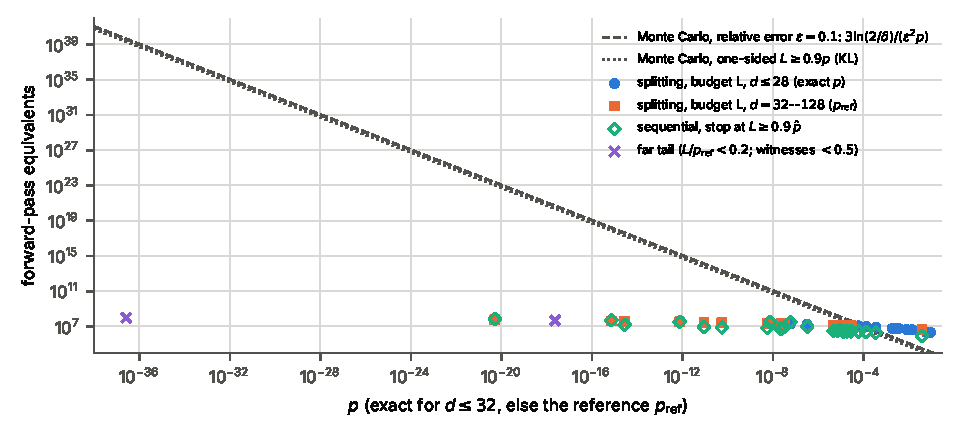
\includegraphics[width=\textwidth]{figures/fig_nets_smc.pdf}
\caption{Cost of the splitting lower bound (fpe, budget L or sequential with target
$0.9$) against $p$, with the Monte Carlo yardsticks. Ratios reached are in
\cref{tab:nets-smc-suite,tab:nets-smc-scaling}; the crosses are the far-tail nets,
whose references are themselves uncertain.}
\label{fig:nets-smc}
\end{figure}

\subsection{Exact counts and certificates of zero: certified partitions}\label{sec:nets-partitions}

A \emph{certified partition} is a decision tree over input coordinates (so its leaves
are subcubes $Q=\{x:x_F=\sigma\}$ with free coordinates $R$, $|R|=r$) whose leaves are
labelled SAFE (with a certificate that $F\ge t$ on $Q$), FAIL ($F<t$ on $Q$), ENUM
(enumerate $Q$) or OPEN; the verifier outputs
$[(\mathcal F+|U|\ell)/2^d,(\mathcal F+|U|u)/2^d]$, with $\mathcal F$ the number of
failing inputs in FAIL and ENUM leaves, $U$ the union of OPEN leaves, and $[\ell,u]$
the KL interval for the failing fraction of uniform samples from $U$. Certificates come
in two kinds, both checked in outward-rounded interval arithmetic. A \emph{linear}
certificate fixes, for each unit relaxed from below, a slope $\alpha\in[0,1]$ (any value
is valid; the verifier clips), and relaxes units from above by chords, as in CROWN
\cite{zhang2018crown}; the verifier recomputes everything else. A \emph{degree-2}
certificate fixes, for each first-layer unit, the parameters of a convex quadratic $q_j$
below or above $\mathrm{relu}$ on its interval (the verifier computes $q_j$ from them
and proves its validity), and a vector $\mu$ and shift $s$ for the S-lemma step
below.

\begin{proposition}[certified partitions]\label{prop:partition}
\begin{enumerate}[label=(\alph*)]
\item (Soundness.) For every net and every argument, the output contains $p$ with
probability at least $1-\delta$; without OPEN leaves it is $p$ exactly. The argument has
the structure of a \textup{\textsc{pcis}} argument (\cref{def:pcis}):
\textup{\textsc{split}} nodes, deterministic leaves whose refutations are linear or
degree-2 certificates or enumeration in place of $P$-refutations, and one envelope node
$\varphi=\one_U$ over the union of the OPEN leaves, which lie in different branches of
the tree (no rule of \cref{def:pcis} forms such a node, so \cref{thm:pcis-sound} does
not apply literally). Soundness is proved directly below, and the sampled part costs
what \cref{thm:envelope}(iv) charges for the looseness $|U|/(2^dD(C\wedge U))$.
\item (Ideal size.) If $C$ has $\mathcal F\ge1$ failing inputs, a tree whose leaves are
all pure (failure-free subcubes or single failing points) with at most
$2\mathcal F(d-\lfloor\log_2\mathcal F\rfloor+1)$ nodes exists; for $p=0$ one node
suffices. Deciding whether a leaf is pure is $\coNP$-complete already for the nets of
\cref{prop:nets-hard}(a), so \cref{thm:ma} bites through the leaf checks, not through
the length of the tree.
\item (Relaxation gap, one hidden layer.) Let $f=c+\sum_ja_j\mathrm{relu}(w_j\cdot x+b_j)$
and let $\mathrm{lb}$ be the linear bound on $Q$ with slopes $\alpha_j=\one[U_j\ge-L_j]$
for the unstable units with $a_j>0$ (CROWN's choice) and chords for those with $a_j<0$,
where $[L_j,U_j]$ is the range of $z_j$ on $Q$. Then
\[
\min_QF-\mathrm{lb}\le\sum_{j\ \text{unstable on }Q}c_j|a_j|\,\|w_{j,R}\|_1,\qquad
c_j=1\ (a_j>0),\quad c_j=\tfrac12\ (a_j<0),
\]
so a SAFE certificate exists as soon as the margin $\min_QF-t$ exceeds the right-hand
side (plus the verifier's outward-rounding slack, and the prover's acceptance margin of
$2^{-30}$ times a bound on $|f|$).
\end{enumerate}
\end{proposition}

\begin{proof}
(a) The verifier parses the tree itself: every split must be on a free coordinate of
its node and have two children, so the leaves partition the cube; their sizes are
summed as integers, and a malformed tree yields $[0,1]$. \emph{Linear certificates.}
Work backwards from an affine lower bound $f\ge G\cdot h_\ell+c$ in the post-activations
of layer $\ell$ (initially $G=w_L$, $c=b_L$), valid on $Q$, given intervals
$L\le z\le U$ for the pre-activations $z=W_\ell h_{\ell-1}+b_\ell$ valid on $Q$. For a
stable unit, $h_j=z_j$ ($L_j\ge0$) or $h_j=0$ ($U_j\le0$). For an unstable unit with
$G_j\ge0$ use $h_j\ge\alpha_jz_j$, valid for every real $z_j$ and $\alpha_j\in[0,1]$; with
$G_j<0$ use $h_j\le\lambda_j(z_j-L_j)$ with $\lambda_j\ge U_j/(U_j-L_j)$, valid on $[L_j,U_j]$
because $\mathrm{relu}$ is convex and below its chord there; if the sign of $G_j$ is not
certain, use $0\le h_j\le U_j$, i.e.\ $G_jh_j\ge\min(G_j,0)U_j$. Each step keeps an
affine lower bound valid on $Q$, now in $h_{\ell-1}$; at the input layer it is affine in
$x$, and its minimum over the box of $Q$, attained at a vertex, is its minimum over $Q$.
The intervals of hidden layers are computed by the same recursion, so the induction is
over layers. A FAIL certificate is the mirror image for $-f$. Evaluating all this in
outward-rounded interval arithmetic (each operation enclosed by the neighbouring doubles
of its result, each matrix product by Higham's bound with the underflow term carried
through later products) makes the computed bound a bound on the exact one.
\emph{Degree-2 certificates.} The layers after the first are relaxed linearly first,
exactly as in a linear certificate; $G_j$ is the resulting (enclosed) coefficient of
$h_j=\mathrm{relu}(z_j)$ for a first-layer unit $j$, and a unit whose $G_j$ has
uncertain sign gets $q_j=0$ and the charge $G_{{\rm lo},j}U_j$, as above. For
$G_j\ge0$ the verifier needs $q_j\le\mathrm{relu}$ on $[L_j,U_j]$ and for $G_j\le0$
$q_j\ge\mathrm{relu}$ there. It accepts only convex $q_j$ (curvature $\kappa_j\ge0$),
and checks, in interval arithmetic: for a minorant, $q_j(L_j)\le0$, $q_j(0)\le0$ and
$q_j(U_j)\le U_j$, which suffice because a convex function on an interval is at most
the larger of its two endpoint values (apply this to $q_j$ on $[L_j,0]$ and to $q_j-z$
on $[0,U_j]$); for a majorant, $q_j(L_j)\ge0$ and $q_j'(L_j)\ge0$ (so
$q_j\ge0$ on $[L_j,U_j]$ by convexity), and either $(q_j-z)(U_j)\ge0$ and
$(q_j-z)'(U_j)\le0$, or $(q_j-z)(0)\ge0$ and $(q_j-z)'(0)\ge0$ (so $q_j\ge z$ on
$[0,U_j]$, again by convexity). A unit whose check fails gets the always valid
$q_j=0$ from below or the chord from above. Then $f\ge Y^\top MY$ on $Q$ for
$Y=(1,x_R)$ and a symmetric $M$ the verifier computes. If
$M-\mathrm{diag}(\mu)-sI\succeq0$ then, as $Y_i^2=1$ for every coordinate of $Y$,
$Y^\top MY\ge\sum_i\mu_iY_i^2+s|Y|^2=\sum_i\mu_i+(r+1)s$. Positive semidefiniteness of
every matrix in the entrywise enclosure is checked by one Cholesky factorisation of
$A-cI$, $A$ the midpoint: if it succeeds, $A-cI+\Delta A=\hat R^\top\hat R\succeq0$ with
$\|\Delta A\|_2\le\gamma_{r+2}\,\mathrm{tr}(A)/(1-\gamma_{r+2})$ for $c\ge0$
\cite[Thm.~10.3]{higham2002} (plus underflow terms, and the rounding of forming
$A-cI$, at most $2u$ times its largest diagonal entry in absolute value), and every matrix within
Frobenius distance $\rho$ of $A$ has smallest eigenvalue at least
$c-\|\Delta A\|_2-\rho$ minus these terms by Weyl's inequality, which the verifier
checks to be positive. \emph{Other leaves.} ENUM leaves are counted exactly by \cref{lem:certeval}
with rational re-evaluation of undecided points; a leaf whose certificate fails or is
non-finite is demoted to OPEN. So $p=\mathcal F/2^d+D(C\wedge U)$, and the envelope
$\one_U$ has exact mass $|U|/2^d$ and an exact uniform sampler (a uniform integer below
$|U|$ selects a leaf and an offset), so \cref{thm:envelope}(ii) gives the interval
with probability $1-\delta$. Enumeration makes the proof system complete; checking is
polynomial in the size of the certificates and of the enumerated subcubes.

(b) Split the coordinates in a fixed order and stop at a node when its subcube
contains no failing input or is a single point. Internal nodes are prefixes of length
$k<d$ of failing inputs, at most $\min(2^k,\mathcal F)$ of each length, so there are at
most $\sum_{k=0}^{d-1}\min(2^k,\mathcal F)\le(2^{\lambda+1}-1)+(d-1-\lambda)\mathcal F\le
\mathcal F(d-\lambda+1)-1$ of them, with $\lambda=\lfloor\log_2\mathcal F\rfloor$; a binary
tree has one more leaf than internal nodes. Deciding that a subcube contains no
failing input is in $\coNP$ (a failing input, re-evaluated exactly, refutes it) and
$\coNP$-hard already for the whole cube of the nets $f_\varphi$, by
\cref{prop:nets-hard}(a).

(c) For one hidden layer the bound is $\mathrm{lb}=\min_Qg$ with
$g=c+\sum_ja_j\ell_j(z_j)$, $\ell_j$ the relaxation of unit $j$, and the minimum is
attained at a point $x^*\in Q$. Then $\min_QF-\mathrm{lb}\le F(x^*)-g(x^*)=\sum_ja_j
(\mathrm{relu}(z_j(x^*))-\ell_j(z_j(x^*)))$, where stable units contribute $0$. On
$[L,U]$ with $L<0<U$: for $a_j>0$, $\mathrm{relu}(z)-\alpha z\le\max((1-\alpha)U,-\alpha L)$,
which is $\min(U,-L)\le(U-L)/2$ for CROWN's $\alpha$; for $a_j<0$, the chord minus
$\mathrm{relu}$ is at most its value at $0$, $-LU/(U-L)\le(U-L)/4$. Since $z_j$ ranges
over the centre $\pm\|w_{j,R}\|_1$, $U_j-L_j=2\|w_{j,R}\|_1$.
\end{proof}

Heuristically, a unit is unstable on a random $r$-dimensional subcube with probability
proportional to $\|w_{j,R}\|_1\propto r$, and at the minimiser of the relaxation its
pre-activation deviates from $0$ by about $\|w_{j,R}\|_2\propto\sqrt r$, so the gap
grows like $r^{3/2}$ (bound (c) is the worst case, $r^2$). We measure exponents of
\nnGapExp{} on the one-hidden-layer squared-loss nets, between the heuristic $3/2$ and
the worst case $2$ and closer to the latter, so the heuristic is at best a rough guide
(the gap scan was computed with the previous verifier, \cref{fig:nets-gap}). The margin $\min_QF-t$ shrinks
as $r$ grows, so certified leaves have a bounded number $r^*$ of free inputs and the
tree has about $2^{d-r^*}$ nodes \emph{whatever $p$ is}.

\paragraph{Results} (\cref{tab:nets-exact,tab:nets-zero}, \texttt{experiments/nets\_prover},
\texttt{nets\_verify}). All \nnExactNets{} suite nets with $d\le28$ are counted exactly
(every count equals the enumerated one). The wins are the logistic nets trained past
the point where the margin dominates: \texttt{bce\_d28\_w32\_s100} ($p=\nnSmallBP$, two
failing inputs) is certified with \nnCertBNodes{} nodes and \nnCertBVerFpe{} verifier
fpe, \nnCertBEnd{}\,s end to end (prover and verifier), against \nnCertBEnum{}\,s for
enumeration and about $\nnCertBMcHours$ hours ($\nnCertBMcFpe$ samples) for Monte Carlo;
\texttt{bce\_d28\_w32\_s150} is certified to have $p=0$ with \nnCertZeroNodes{} nodes,
$\nnCertZeroFpe$ fpe, in \nnCertZeroEnd{}\,s, which Monte Carlo can never do. For
squared loss at $d=24$ the certificate is only \nnEnumOverCertMse{} times cheaper than
enumerating the cube in fpe, and in seconds enumeration (\nnEnumSecMse{}\,s) beats
prover plus verifier (\nnEndSecMse{}\,s) on every $d=24$ net: the numpy verifier costs
\nnVerUsPerFpe{}\,$\mu$s per fpe, against \nnMcUsPerSample{}\,$\mu$s per Monte Carlo
sample. Branch and bound without a prover (CROWN bounds, \texttt{nets\_verify}) counts
exactly on \nnBabExactRuns{} of the \nnBabRuns{} one-hidden-layer nets (the other two end
with \nnBabAmb{} undecided points, and their intervals contain $p$), at \nnBabEnumMse{}
times the cost of enumeration for squared loss and \nnBabEnumBce{} for logistic loss.
These ratios are in branch and bound's own cost model, in which enumerating the cube costs
$\nnBabEnumTwoFour$ fpe at $d=24$ and $\nnBabEnumTwoEight$ at $d=28$; the enumeration column
of \cref{tab:nets-exact} is in the certified-partition verifier's cost model, which
counts fewer flops per point. Branch and bound spends \nnBabWallFactor{} times the
wall-clock of a Monte Carlo sample per fpe, in the same process. Degree-2 leaves make trees \nnQuadNodeRatio{} times
smaller but cost \nnQuadFpeRatio{} times more fpe and \nnQuadSecRatio{} times more
seconds to verify. Two hidden layers defeat both: no certificate is planned cheaper
than enumeration (\nnDeepEnumSec{}\,s), and branch and bound leaves upper ends of
\nnBabDeepHi{} after its time limit. A perfect engine, deciding every pure subcube at
once, would need \nnOracleRatio{} times fewer nodes than CROWN's tree (for the
\nnSmallDF{} failures of \texttt{mse\_d24\_w32\_s1500}: \nnOracleOneFiveNodes{} nodes,
within the bound \nnOracleOneFiveBound{} of (b), against \nnCrownOneFiveNodes{}), and
greedily grown failing subcubes have dimension at most \nnMaxFailDim{}: the obstacle is
deciding SAFE, not the geometry of the failures.

\emph{Certificates of $p=0$.} Of \nnZeroNets{} one-hidden-layer nets trained for at
least $1000$ (squared loss) or $300$ (logistic loss) steps, \nnZeroZero{} are certified
to have $p=0$ (\cref{tab:nets-zero}), \nnZeroPos{} have $p>0$ and are counted exactly,
and \nnZeroOpen{} at $d=40$--$64$ remain open. Longer
training makes certification nearly free (about $\nnRootFpe$ fpe and $\nnRootSec$\,s, at
the root, for some nets up to $d=32$ with squared and $d=40$ with logistic loss); at $d=48$ and $64$ it costs $\nnZeroFpeFortyEight$
and $\nnZeroFpeSixtyFour$ fpe ($\nnZeroSecFortyEight$ and $\nnZeroSecSixtyFour$\,s). Monte
Carlo with $10^7$ samples only shows $p\le\nnMcUpperTenSeven$. For the suite net
\texttt{bce\_d64\_w64\_s1000} we attempted the whole certificate within
$\nnSixFourBudgetMin$ minutes on \nnSixFourWorkers{} worker processes: \nnSixFourDone{} of its \nnSixFourTotal{} top-level pieces, chosen in
random order, were certified exactly, all with no failing input, so \nnSixFourFrac{} of
the cube is certified failure-free ($\nnSixFourNodes$ nodes, $\nnSixFourFpe$ verifier
fpe; $\nnSixFourProverSec$\,s of proving and $\nnSixFourVerSec$\,s of verifying summed
over the workers, $\nnSixFourWall$\,s of wall-clock). Extrapolating from these uniformly
sampled pieces, the whole certificate has $\nnSixFourEstNodes\pm\nnSixFourEstNodesSe$
nodes and costs $\nnSixFourEstFpe\pm\nnSixFourEstFpeSe$ verifier fpe; as many Monte
Carlo samples would only show $p\le\nnSixFourMcUpper$. For the other $d=64$ suite nets
the estimated certificates cost $\nnKnA$ (\texttt{bce\_d64\_w64\_s300}) to $\nnKnE$ fpe
(\texttt{mse\_d64\_w64\_s300}, more than the $\nnKnEnum$ of enumeration).

\begin{table}[tbp]
\centering\scriptsize\setlength{\tabcolsep}{3pt}
\resizebox{\textwidth}{!}{\begin{tabular}{lrrlrrrrr}
\toprule
net & $p$ & $F$ & argument & verifier fpe\,(s) & prover s & B\&B fpe\,(s) & enumeration fpe\,(s) & Monte Carlo fpe\,(s)\\
\midrule
\texttt{mse\_d24\_w32\_s300} & $0.071$ & 1193958 & 42227 nodes & $1.3\cdot10^{6}$\,($7.2$) & 110 & $7.3\cdot10^{6}$\,($10$) & $1.3\cdot10^{6}$\,($5.4$) & $1.6\cdot10^{4}$\,($0.012$)\\
\texttt{mse\_d24\_w32\_s600} & $8.3\cdot10^{-3}$ & 138936 & 177329 nodes & $1.2\cdot10^{6}$\,($7.5$) & 76 & $5.7\cdot10^{6}$\,($7.2$) & $1.3\cdot10^{6}$\,($5.1$) & $1.3\cdot10^{5}$\,($0.11$)\\
\texttt{mse\_d24\_w32\_s1000} & $3.6\cdot10^{-4}$ & 6012 & 305973 nodes & $8.7\cdot10^{5}$\,($8.0$) & 49 & $3.7\cdot10^{6}$\,($4.3$) & $1.3\cdot10^{6}$\,($5.2$) & $3.1\cdot10^{6}$\,($2.3$)\\
\texttt{mse\_d24\_w32\_s1500} & $9.7\cdot10^{-6}$ & 163 & 253127 nodes & $5.4\cdot10^{5}$\,($5.0$) & 29 & $2.4\cdot10^{6}$\,($2.6$) & $1.3\cdot10^{6}$\,($5.8$) & $1.1\cdot10^{8}$\,($94$)\\
\texttt{mse\_d24\_w32\_s2000} & $6\cdot10^{-8}$ & 1 & 160647 nodes & $3.2\cdot10^{5}$\,($2.4$) & 16 & $1.4\cdot10^{6}$\,($1.5$) & $1.3\cdot10^{6}$\,($5.2$) & $1.9\cdot10^{10}$\,($1.2\cdot10^{4}$)\\
\texttt{mse\_d28\_w64\_s300} & $0.013$ & 3468961 & [ENUM] & $1.9\cdot10^{7}$\,($150$) & 1.3 & $1.1\cdot10^{8}$\,($120$)$^{\ast}$ & $1.9\cdot10^{7}$\,($150$) & $8.6\cdot10^{4}$\,($0.098$)\\
\texttt{mse\_d28\_w64\_s600} & $6\cdot10^{-5}$ & 16155 & [ENUM] & $1.9\cdot10^{7}$\,($150$) & 1.1 & $9\cdot10^{7}$\,($98$) & $1.9\cdot10^{7}$\,($150$) & $1.8\cdot10^{7}$\,($18$)\\
\texttt{mse\_d28\_w64\_s1000} & $3.3\cdot10^{-7}$ & 89 & [ENUM] & $1.9\cdot10^{7}$\,($150$) & 1.5 & $6.8\cdot10^{7}$\,($73$) & $1.9\cdot10^{7}$\,($150$) & $3.3\cdot10^{9}$\,($3300$)\\
\texttt{mse\_d28\_w64\_s1500} & $0$ & 0 & 4983651 nodes, 32 pieces & $10^{7}$\,($130$) & 800 & $4.4\cdot10^{7}$\,($47$) & $1.9\cdot10^{7}$\,($140$) & cannot certify 0\\
\texttt{bce\_d28\_w32\_s30} & $1.9\cdot10^{-3}$ & 507779 & 1201597 nodes & $3.4\cdot10^{6}$\,($39$) & 210 & $1.4\cdot10^{7}$\,($16$)$^{\ast}$ & $1.9\cdot10^{7}$\,($71$) & $5.9\cdot10^{5}$\,($0.36$)\\
\texttt{bce\_d28\_w32\_s60} & $1.3\cdot10^{-5}$ & 3543 & 237621 nodes & $5\cdot10^{5}$\,($5.9$) & 31 & $3.5\cdot10^{6}$\,($3.4$) & $1.9\cdot10^{7}$\,($65$) & $8.4\cdot10^{7}$\,($75$)\\
\texttt{bce\_d28\_w32\_s100} & $7.5\cdot10^{-9}$ & 2 & 20789 nodes & $4.1\cdot10^{4}$\,($0.31$) & 3.9 & $8.2\cdot10^{5}$\,($0.69$) & $1.9\cdot10^{7}$\,($69$) & $1.5\cdot10^{11}$\,($1.2\cdot10^{5}$)\\
\texttt{bce\_d28\_w32\_s150} & $0$ & 0 & 2061 nodes & $4100$\,($0.032$) & 1.4 & $2.3\cdot10^{5}$\,($0.17$) & $1.9\cdot10^{7}$\,($74$) & cannot certify 0\\
\midrule
two hidden layers (8 nets) & $0$--$0.093$ & & [ENUM] & $1.5\cdot10^{8}$--$1.9\cdot10^{8}$\,($190$--$500$) & & \multicolumn{3}{l}{B\&B: upper end $0.78$--$0.91$ after 940--2600\,s (4 nets)}\\
\bottomrule
\end{tabular}
}
\caption{Exact counts at $d\le28$ ($\delta=0.05$, $\eps=0.1$ for Monte Carlo, whose
seconds are at the median measured time per sample of the net, as in
\cref{tab:nets-smc-suite}). Argument:
the certified partition built by the prover, or [ENUM] when its plan put the
certificate above a fixed fraction of the cost of enumeration. B\&B: branch and
bound with CROWN bounds and no prover; $^\ast$ marks the two runs that ended with
\nnBabAmb{} undecided points, whose intervals contain $p$ (\texttt{nets\_prover/run\_suite.py},
\texttt{nets\_verify/exp\_suite.py}, \texttt{wallclock.py}).}
\label{tab:nets-exact}
\end{table}

\begin{table}[htbp]
\centering\scriptsize
\begin{tabular}{lrrrrrrr}
\toprule
loss & $d$ & nets & $p=0$ certified & $p>0$ exact & open & at the root & median fpe\,(s)\\
\midrule
squared & 12 & 15 & 15 & 0 & 0 & 0 & $2800$\,($4\cdot10^{-3}$)\\
squared & 16 & 15 & 14 & 1 & 0 & 2 & $7900$\,($9\cdot10^{-3}$)\\
squared & 20 & 15 & 15 & 0 & 0 & 4 & $7800$\,($0.010$)\\
squared & 24 & 15 & 13 & 2 & 0 & 2 & $2.6\cdot10^{4}$\,($0.031$)\\
squared & 28 & 10 & 8 & 2 & 0 & 3 & $1.1\cdot10^{5}$\,($0.11$)\\
squared & 32 & 10 & 10 & 0 & 0 & 3 & $2.9\cdot10^{5}$\,($0.38$)\\
squared & 40 & 3 & 2 & 0 & 1 & 0 & $3300$\,($8\cdot10^{-3}$)\\
squared & 48 & 3 & 2 & 0 & 1 & 0 & $3.2\cdot10^{7}$\,($40$)\\
squared & 64 & 3 & 1 & 0 & 2 & 0 & $3.7\cdot10^{7}$\,($49$)\\
logistic & 16 & 6 & 6 & 0 & 0 & 3 & $140$\,($2\cdot10^{-3}$)\\
logistic & 24 & 6 & 6 & 0 & 0 & 2 & $3600$\,($8.5\cdot10^{-3}$)\\
logistic & 32 & 3 & 3 & 0 & 0 & 2 & $4.9$\,($10^{-3}$)\\
logistic & 40 & 3 & 3 & 0 & 0 & 1 & $5.2\cdot10^{6}$\,($7.0$)\\
\bottomrule
\end{tabular}

\caption{Frequency and cost of certificates of $p=0$ (one hidden layer of width $32$,
trained for at least $1000$ squared-loss or $300$ logistic-loss steps; branch and bound
with CROWN bounds, at most \nnZeroLimit\,s per net; \texttt{nets\_verify/exp\_zero.py}). ``At the root'':
certified with a single bound.}
\label{tab:nets-zero}
\end{table}

\begin{figure}[htbp]
\centering
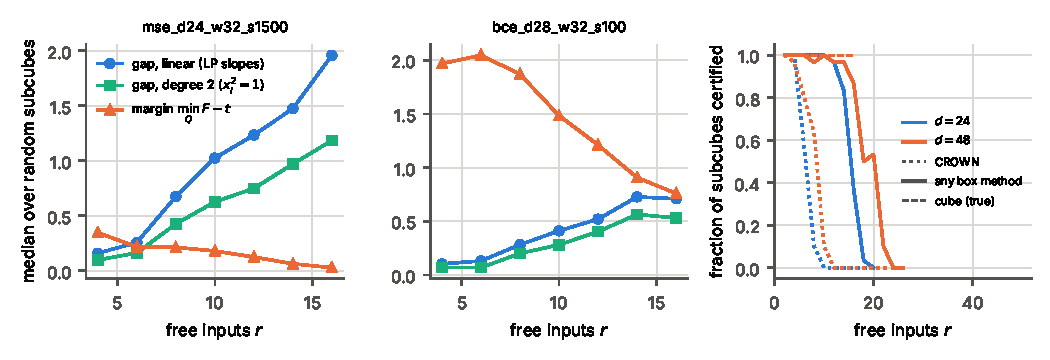
\includegraphics[width=\textwidth]{figures/fig_nets_gap.pdf}
\caption{Left and middle: median gap between the exact minimum of $F$ on random
$r$-dimensional subcubes and the certified bound, linear and degree-2, against the
margin $\min_QF-t$ (\texttt{nets\_prover/gap\_scan.py}, computed with the previous
verifier, whose bounds agree with the current ones far below the scale shown). Right: fraction of
subcubes certified by CROWN, by any method valid on the subcube's box (exact box
minimum by MILP, witnesses re-evaluated), and true on the cube, for squared-loss nets
of width $32$ trained for $1500$ steps (\texttt{nets\_verify/exp\_barrier.py}).}
\label{fig:nets-gap}
\end{figure}

\begin{figure}[htbp]
\centering
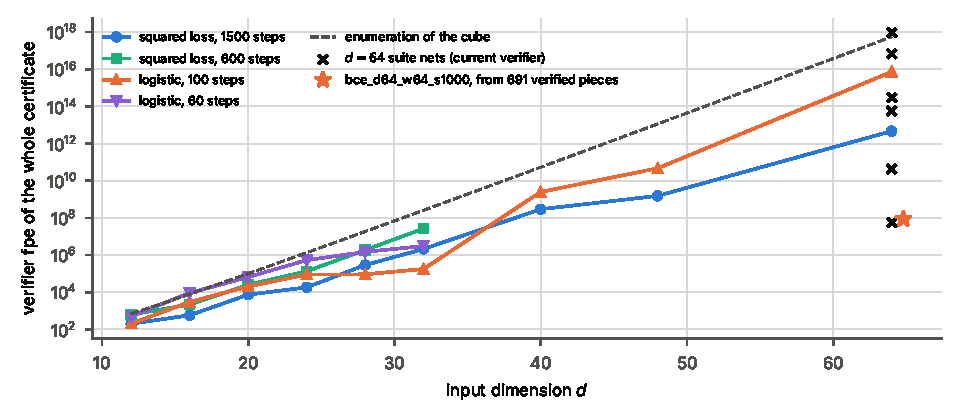
\includegraphics[width=\textwidth]{figures/fig_nets_knuth.pdf}
\caption{Verifier cost of the whole certified partition against $d$ (Knuth estimates
\cite{knuth1975} from random root-to-leaf probes of the prover's tree, medians over
\nnKnuthSeeds{} seeds, in the previous verifier's cost model, which counts fewer flops
per leaf than the current one; \texttt{nets\_prover/scaling.py}), the $d=64$ suite nets with the current
verifier (\texttt{knuth\_d64.py}), and the extrapolation from the certified pieces of
\texttt{bce\_d64\_w64\_s1000} (\texttt{full\_d64.py}). The fitted growth is
$2^{(\nnKnuthSlopesMse)d}$ for the two squared-loss families and
$2^{(\nnKnuthSlopesBce)d}$ for the two logistic ones.}
\label{fig:nets-knuth}
\end{figure}

\subsection{Why upper bounds fail on trained squared-loss nets}\label{sec:nets-barriers}

By \cref{thm:blackbox} an upper bound below the sampling scale needs deduction about
the weights. For squared-loss nets three barriers explain why every deduction we
could make cheap fails, and \cref{tab:nets-barriers} measures them on all
\nnBarNets{} suite nets. Extend $F$ to the box $[-1,1]^d$ by the same formula.

\begin{proposition}[box barrier]\label{prop:boxbarrier}
Suppose $F(0)<t$.
\begin{enumerate}[label=(\alph*)]
\item Every function $B\le F$ on $[-1,1]^d$ has $B(0)<t$, so no bound valid on the
box (interval arithmetic, CROWN, any LP or convex relaxation, MILP over the box,
Lipschitz bounds) certifies $F\ge t$ on the cube; the same holds for a subcube whose
centre has $F<t$. More generally, the same holds, without assuming $F(0)<t$, as soon as
$F(y)<t$ at some point $y$ of the box (of the subcube's box).
\item Let $\Phi:[-1,1]^d\to\R_{\ge0}$ be convex in each coordinate separately (e.g.\ a
positive combination of exponentials of affine functions, or a product of such with
factors $1+e^{\alpha_jz_j}$) with $\Phi\ge1$ wherever $F<t$ on the box. Then
$Z=\E_D\Phi\ge\Phi(0)\ge1$, so the envelope $\Phi$ has looseness $K\ge1/p$.
\end{enumerate}
\end{proposition}

\begin{proof}
(a) $B(0)\le F(0)<t$; for a subcube, its box contains its centre; and in general
$B(y)\le F(y)<t$. (b) For $x$ uniform
on $\{\pm1\}^d$, convexity in $x_1$ gives $\E_{x_1}\Phi(x_1,y)\ge\Phi(0,y)$ for every
$y$, and inducting over the coordinates, $\E_D\Phi\ge\Phi(0)$; since $F(0)<t$,
$\Phi(0)\ge1$. A product of positive log-convex functions is log-convex, hence convex,
which covers the examples.
\end{proof}

The extreme small-ball point is the centre: $F(0)=c+\sum_ja_j\mathrm{relu}(b_j)$ has
every $|z_j|$ as small as the biases allow. The barrier covers the tilts and the
sign-pattern envelopes we built; it does not cover cell-based envelopes from a dynamic
program over a few hidden forms (which are not functions on the box; a constructed
small-ball net has one with $Z<1$), enumeration, exact optimisation over the cube, or
arguments using $x_i^2=1$, such as the degree-2 certificates above.

\begin{proposition}[cube barrier]\label{prop:cubebarrier}
If $g_0+\gamma\cdot x\le F(x)$ for all $x\in\{\pm1\}^d$, then
$g_0\le s^*=\min_x\frac12(F(x)+F(-x))$. Hence the tilted envelope
$\varphi(x)=e^{\theta(t-g_0-\gamma\cdot x)}$ ($\theta\ge0$), which dominates $[F<t]$ on the
cube, has mass $Z=e^{\theta(t-g_0)}\prod_i\cosh(\theta\gamma_i)\ge e^{\theta(t-s^*)}$,
which is at least $1$ when $s^*\le t$, however the minorant was certified.
\end{proposition}

\begin{proof}
Add the inequalities at $x$ and $-x$: $2g_0\le F(x)+F(-x)$. The mass is a product over
independent coordinates, and $\cosh\ge1$.
\end{proof}

\begin{proposition}[decoupling floor]\label{prop:decoupling}
Let $F=\sum_{k=1}^mF_k$, $\theta\ge0$ and $q_1,\dots,q_m\ge1$. Every bound of the form
$p\le e^{\theta t}\prod_k\|e^{-\theta F_k}\|_{q_k}$ (the generalised Hölder inequality,
with $\sum_k1/q_k=1$; Finner's inequality \cite{finner1992}, for parts depending on
overlapping sets of independent coordinates) is at least
$\inf_{\theta\ge0}e^{\theta t}\prod_k\E e^{-\theta F_k}$, the Chernoff bound the parts would
give if they were independent.
\end{proposition}

\begin{proof}
For $Y\ge0$ and $q\ge1$, $\|Y\|_q\ge\|Y\|_1=\E Y$ (Jensen), so each bound is at least
$e^{\theta t}\prod_k\E e^{-\theta F_k}$ at its $\theta$.
\end{proof}

With the hidden units as parts, the independent-parts floor is \nnFloorMse{} on the
one-hidden-layer squared-loss nets with $d\le28$, whose $p$ ranges over \nnPmse{}: the
even parts of positive- and negative-weight units cancel (correlation \nnCorrEvenPM{}),
so the true lower tail is far thinner than independence predicts. This is the
opposite of the unate case of \cref{thm:janson}, where positive correlation makes the
independence estimate a certified lower bound. Measured on the suite
(\cref{tab:nets-barriers}): $F(0)<t$ on all \nnMseSmallD{} squared-loss nets with
$d\le28$; $s^*<t$ on \nnSymNeg{} of the \nnMsePos{} with $p>0$ (the exception has
$s^*-t=\nnSymExc$); the best certified Hölder bound is \nnHolderMse{} and McDiarmid
\nnMcdMse{} there, and McDiarmid is at least \nnMcdAll{} on every net; the best box
tilt has $\log Z\ge0$ on all \nnTiltAll{} nets (its optimiser ends at $\theta\to0$, i.e.\
at Monte Carlo); bounding the positive units alone, even with their exact law, cannot
go below \nnQplus{}; and CROWN's median gap on $8$-dimensional subcubes exceeds the
median margin on \nnGapExceedsMse{} of the \nnMseSmallD{} squared-loss nets with
$d\le28$, so its $r_{50}$ (the largest subcube dimension at which half of the random
subcubes are certified) is small. The ideal Chernoff envelope $e^{\theta(t-F)}$ would have
$K=\nnKideal{}$: the obstacle is computing its mass and sampling it, not information.

Methods with an oracle that optimises over the cube escape the box barrier, at
verification cost. Perturb-and-MAP \cite{hazan2012} certifies $U=\nnPmAU$ at
$p=\nnPmAP$ and $\nnPmBU$ at $p=\nnPmBP$ (\nnPmACalls{} MAP calls each, $\nnPmASec$ and
$\nnPmBSec$\,s) and $\nnPmCU$ at $p=\nnPmCP$ (\nnPmCCalls{} calls, $\nnPmCSec$\,s); on the suite nets with $p\le10^{-4}$ it certifies $U=p^c$
with $c=\nnPmExp$; the cube-certified tilt exists only
when $s^*>t$, and on \texttt{mse\_d24\_w32\_s2000} has $Z=\nnCubeZ$, $K=\nnCubeK$ and gives
$[\nnCubeLo,\nnCubeHi]$ from $\nnCubeSamples$ samples, against $\nnCubeMc$ for Monte
Carlo, after \nnCubeCalls{} MAP calls ($\nnCubeSec$\,s in all). Each call is $\NP$-hard; we answered them by
enumeration, so these certificates cost more than computing $p$, and a MILP solver
leaves gaps of \nnMapGaps{} nats on the $d=64$, width-64 suite nets after
$\nnMapSec$\,s.
The one large-margin success needs no oracle: on \texttt{bce\_d64\_w64\_s1000}
($F(0)-t=\nnLargeMarginFzero$, and the solver's box minimum is $t+\nnLargeMarginBox$)
the sign-pattern envelope, with \nnSignSplit{} negative units split, has $Z=\nnSignZ$,
and $\nnSignSamples$ samples certify $p\le\nnSignHi$, against $\nnSignMc$ for Monte
Carlo with the same samples ($\nnSignSec$\,s in all). No net with $d\le30$ is in this
regime, so it is not checked against an exact $p$.

\begin{table}[tbp]
\centering\scriptsize\setlength{\tabcolsep}{3pt}
\resizebox{\textwidth}{!}{\begin{tabular}{lrrrrrrrrrrr}
\toprule
net & $p$ & $F(0)-t$ & $\min_{\rm box}F-t$ & $s^*-t$ & floor & $U_{\rm H\ddot older}$ & $\log Z_{\rm tilt}$ & $Z_{\rm sign}$ & gap$_8$ & margin$_8$ & $r_{50}$\\
\midrule
\texttt{mse\_d24\_w32\_s300} & $0.071$ & $-0.196$ & $-1.317$ & $-1.040$ & $0.47$ & 0.974 & $4\cdot10^{-5}$ & $\geq1$ & 1.01 & $-0.19$ & 2\\
\texttt{mse\_d24\_w32\_s600} & $8.3\cdot10^{-3}$ & $-0.152$ & $-0.827$ & $-0.515$ & $0.38$ & 0.966 & $3\cdot10^{-5}$ & $\geq1$ & 0.96 & $0.03$ & 2\\
\texttt{mse\_d24\_w32\_s1000} & $3.6\cdot10^{-4}$ & $-0.108$ & $-0.581$ & $-0.240$ & $0.31$ & 0.959 & $3\cdot10^{-5}$ & $\geq1$ & 0.87 & $0.17$ & 4\\
\texttt{mse\_d24\_w32\_s1500} & $9.7\cdot10^{-6}$ & $-0.064$ & $-0.412$ & $-0.090$ & $0.24$ & 0.951 & $3\cdot10^{-5}$ & $\geq1$ & 0.80 & $0.24$ & 4\\
\texttt{mse\_d24\_w32\_s2000} & $6\cdot10^{-8}$ & $-0.022$ & $-0.307$ & $0.011$ & $0.18$ & 0.939 & $2\cdot10^{-5}$ & $\geq1$ & 0.72 & $0.29$ & 4\\
\texttt{mse\_d28\_w64\_s300} & $0.013$ & $-0.332$ & $-0.859$ & $-0.623$ & $0.28$ & 0.980 & $5\cdot10^{-5}$ & $\geq1$ & 0.98 & $0.09$ & 2\\
\texttt{mse\_d28\_w64\_s600} & $6\cdot10^{-5}$ & $-0.309$ & $-0.565$ & $-0.230$ & $0.19$ & 0.974 & $4\cdot10^{-5}$ & $\geq1$ & 0.88 & $0.21$ & 4\\
\texttt{mse\_d28\_w64\_s1000} & $3.3\cdot10^{-7}$ & $-0.277$ & $-0.431$ & $-0.059$ & $0.13$ & 0.968 & $4\cdot10^{-5}$ & $\geq1$ & 0.82 & $0.26$ & 4\\
\texttt{mse\_d28\_w64\_s1500} & $0$ & $-0.238$ & $-0.349$ & $0.040$ & $0.063$ & 0.956 & $3\cdot10^{-5}$ & $\geq1$ & 0.69 & $0.32$ & 4\\
\texttt{mse\_d28\_w32x32\_s100} & $0.060$ & $-0.397$ & $-0.970$ & $-0.634$ & - & - & $4\cdot10^{-3}$ & - & 2.15 & $-0.17$ & 2\\
\texttt{mse\_d28\_w32x32\_s200} & $0.015$ & $-0.359$ & $-0.909$ & $-0.420$ & - & - & $4\cdot10^{-3}$ & - & 1.77 & $0.03$ & 2\\
\texttt{mse\_d28\_w32x32\_s300} & $3.6\cdot10^{-3}$ & $-0.319$ & $-0.765$ & $-0.274$ & - & - & $3\cdot10^{-3}$ & - & 1.61 & $0.12$ & 2\\
\texttt{mse\_d28\_w32x32\_s500} & $1.3\cdot10^{-4}$ & $-0.240$ & $-0.576$ & $-0.112$ & - & - & $3\cdot10^{-3}$ & - & 1.37 & $0.19$ & 4\\
\midrule
\texttt{bce\_d28\_w32\_s30} & $1.9\cdot10^{-3}$ & $0.129$ & $-1.286$ & $-0.407$ & $0.020$ & 0.759 & $2\cdot10^{-5}$ & $\geq1$ & 0.71 & $0.62$ & 6\\
\texttt{bce\_d28\_w32\_s60} & $1.3\cdot10^{-5}$ & $0.260$ & $-0.753$ & $0.100$ & $1.1\cdot10^{-3}$ & 0.614 & $10^{-5}$ & $\geq1$ & 0.65 & $1.24$ & 10\\
\texttt{bce\_d28\_w32\_s100} & $7.5\cdot10^{-9}$ & $0.418$ & $-0.390$ & $0.603$ & $2\cdot10^{-5}$ & 0.453 & $7\cdot10^{-6}$ & $\geq1$ & 0.68 & $1.71$ & 12\\
\texttt{bce\_d28\_w32\_s150} & $0$ & $0.591$ & $-0.155$ & $1.011$ & $6.5\cdot10^{-8}$ & 0.317 & $7\cdot10^{-6}$ & $\geq1$ & 0.75 & $2.25$ & 12\\
\texttt{bce\_d28\_w64x64\_s20} & $0.093$ & $0.033$ & $-1.790$ & $-0.795$ & - & - & $9\cdot10^{-3}$ & - & 4.15 & $-0.14$ & 2\\
\texttt{bce\_d28\_w64x64\_s40} & $2.3\cdot10^{-3}$ & $0.074$ & $-1.284$ & $-0.155$ & - & - & $9\cdot10^{-3}$ & - & 4.00 & $0.54$ & 2\\
\texttt{bce\_d28\_w64x64\_s60} & $1.9\cdot10^{-5}$ & $0.118$ & $-0.776$ & $0.335$ & - & - & $9\cdot10^{-3}$ & - & 4.15 & $0.91$ & 4\\
\texttt{bce\_d28\_w64x64\_s100} & $0$ & $0.203$ & $-0.424$ & $1.040$ & - & - & $8\cdot10^{-3}$ & - & 4.09 & $1.86$ & 4\\
\midrule
\texttt{mse\_d64\_w64\_s300} & ? & $-0.318$ & $-1.836$ & $-1.332$$^\ddagger$ & $0.18$ & 0.991 & $8\cdot10^{-5}$ & $\geq1$ & 0.44 & $0.15$ & 4\\
\texttt{mse\_d64\_w64\_s1000} & ? & $-0.207$ & $-0.738$ & $-0.342$$^\ddagger$ & $0.033$ & 0.973 & $5\cdot10^{-5}$ & $\geq1$ & 0.29 & $0.33$ & 8\\
\texttt{mse\_d64\_w64\_s3000} & ? & $0.114$ & $-0.133$ & $0.136$$^\ddagger$ & $2.6\cdot10^{-5}$ & 0.871 & $2\cdot10^{-5}$ & $\geq1$ & 0.14 & $0.42$ & 14\\
\texttt{bce\_d64\_w64\_s100} & ? & $0.463$ & $-2.017$ & $0.149$$^\ddagger$ & $9.9\cdot10^{-7}$ & 0.679 & $5\cdot10^{-5}$ & $\geq1$ & 0.50 & $2.72$ & 16\\
\texttt{bce\_d64\_w64\_s300} & ? & $0.890$ & $-0.786$ & $1.373$$^\ddagger$ & $1.7\cdot10^{-19}$ & 0.427 & $4\cdot10^{-5}$ & $\geq1$ & 0.53 & $4.56$ & 24\\
\texttt{bce\_d64\_w64\_s1000} & ? & $1.520$ & $0.114$$^\dagger$ & $2.554$$^\ddagger$ & $4\cdot10^{-41}$ & 0.220 & $2\cdot10^{-5}$ & $4.9\cdot10^{-3}$ & 0.65 & $6.47$ & 24\\
\texttt{bce\_d128\_w128x128\_s100} & ? & $0.194$ & $-1.164$ & $1.144$$^\ddagger$ & - & - & $0.04$ & - & 1.30 & $4.28$ & 12\\
\texttt{bce\_d128\_w128x128\_s300} & ? & $0.324$ & $-0.711$ & $2.380$$^\ddagger$ & - & - & $0.04$ & - & 1.31 & $6.29$ & 14\\
\texttt{bce\_d128\_w128x128\_s1000} & ? & $0.499$ & $-0.203$ & $4.210$$^\ddagger$ & - & - & $0.03$ & - & 1.35 & $9.69$ & 16\\
\bottomrule
\end{tabular}
}
\caption{Barrier diagnostics (\texttt{nets\_analytic/barrier\_table.py}). $\min_{\rm
box}F-t$: value at a re-evaluated box point found by MILP ($^\dagger$: the solver's
claimed optimum, not certified); $s^*-t$: exact for $d\le28$, else the best value found
($^\ddagger$, an upper bound on $s^*-t$); floor: independent-units Chernoff value
(\cref{prop:decoupling}); $U_{\rm H\ddot older}$: best certified Hölder bound; $\log
Z_{\rm tilt}$: best box-relaxed tilt; $Z_{\rm sign}$: sign-pattern envelope (one hidden
layer); gap$_8$ and margin$_8$: median CROWN gap and margin on $8$-dimensional
subcubes; $r_{50}$: CROWN's certified subcube dimension. ``?'': $p$ unknown; ``-'': not
computed for two hidden layers.}
\label{tab:nets-barriers}
\end{table}

\subsection{Regimes, heuristics, and what remains open}\label{sec:nets-regimes}

\Cref{tab:nets-regimes} collects the regime map. Heuristic estimators are useful
comparators but unsound (\cref{tab:nets-heuristics}, \texttt{experiments/nets\_structure},
\nnHeurPoints{} (net, level) points on \nnHeurNets{} nets with exact $P$): the best,
``select'' (a quadratic fit to the lower tail of $10^5$ samples for one-hidden-layer
squared loss, a sphere-input surrogate otherwise), is within a factor $10$ on
\nnSelWithin{} of points, worst off by $10^{\nnSelWorst}$, and predicts $p=0$ correctly
on \nnSelPzero{} of nets. The presumption of independence over hidden units
overestimates by a median $10^{\nnPoiMedian}$, for the cancellation reason of
\cref{prop:decoupling}. Nets of the same architecture break all of them: the output
Gaussian is off by $10^{\nnLatticeOff}$ on a lattice small ball at $d=\nnLatticeD$, and
the tail fit misses a planted $2^{-16}$ subcube by $10^{\nnPlantMcfitOff}$.

Tried without gain: soft (tempered) levels, block-Gibbs moves and selection pooled over
trajectories; explicit self-certifying proposals (autoregressive and kernel-mixture
models fitted to splitting samples); McDiarmid, Esseen/Halász-type and exact-moment
bounds; envelopes over a few hidden forms; and quadratic and LP-dual branch-and-bound
prototypes.

\begin{table}[htbp]
\centering\scriptsize\setlength{\tabcolsep}{4pt}
\begin{tabular}{p{2.1cm}p{2.8cm}p{3.0cm}p{3.5cm}p{3.1cm}}
\toprule
{\raggedright regime\par} & {\raggedright best sound two-sided\par} & {\raggedright best sound lower bound\par} & {\raggedright exact or $p=0$ certificate\par} & {\raggedright cost against Monte Carlo\par}\\
\midrule
{\raggedright $p\gtrsim10^{-3}$, any $d$\par} & {\raggedright Monte Carlo\par} & {\raggedright Monte Carlo\par} & {\raggedright enumeration at $d\lesssim30$, else none\par} & {\raggedright Monte Carlo $8$--$130$ times cheaper than splitting (fpe)\par}\\
{\raggedright $d\lesssim30$, $p>0$\par} & {\raggedright exact count (enumeration, B\&B, certified partition)\par} & {\raggedright witness list (exact when $F$ is small), splitting\par} & {\raggedright certified partition, B\&B\par} & {\raggedright verifier $210$, $5.8\cdot10^{4}$, $3.6\cdot10^{6}$ times cheaper in fpe at $p=9.7\cdot10^{-6}$, $6\cdot10^{-8}$, $7.5\cdot10^{-9}$; end to end in seconds $2.8$, $660$, $2.9\cdot10^{4}$\par}\\
{\raggedright $d\geq40$, $p>0$, large failure set\par} & {\raggedright Monte Carlo only (squared loss: \cref{sec:nets-barriers})\par} & {\raggedright splitting, $L/p_{\rm ref}=0.87$--$0.97$\par} & {\raggedright none within reach (whole certificate $5.7\cdot10^{13}$--$9.5\cdot10^{17}$\,fpe at $d=64$)\par} & {\raggedright lower bound $3.8$--$10^{15}$ times cheaper for $p_{\rm ref}\leq10^{-4}$ (fpe, KL yardstick)\par}\\
{\raggedright $p=0$, or a large margin\par} & {\raggedright certificate of $p=0$; sign-pattern envelope (one $d=64$ net)\par} & {\raggedright -- ($L=0$ is right)\par} & {\raggedright 98 of 107 nets certified; at $d=64$, 67.5\% of the cube in $110$\,min\par} & {\raggedright Monte Carlo never certifies $p=0$\par}\\
{\raggedright far tail, $z\gtrsim7.8$\par} & {\raggedright none\par} & {\raggedright witness list ($0.42$--$0.47$ of $p_{\rm ref}$); splitting alone $0.17$--$0.18$\par} & {\raggedright only with a large margin\par} & {\raggedright --\par}\\
\bottomrule
\end{tabular}

\caption{Regime map for the suite and the nets trained here. Costs as in
\cref{tab:nets-smc-suite,tab:nets-smc-scaling,tab:nets-exact}.}
\label{tab:nets-regimes}
\end{table}

\begin{table}[htbp]
\centering\scriptsize
\begin{tabular}{lrrrrrr}
\toprule
estimator & median & median $|\cdot|$ & $\times10$ & $\times10$, $P\leq10^{-6}$ & worst & $p=0$ right\\
\midrule
select & $0.04$ & 0.18 & 95\% & 87\% & 3.3 & 98\%\\
tail fit & $0.07$ & 0.18 & 93\% & 72\% & 7.5 & 96\%\\
sphere surrogate & $0.24$ & 0.36 & 77\% & 71\% & 5.7 & 94\%\\
output Gaussian & $0.28$ & 0.68 & 63\% & 35\% & 43.1 & 90\%\\
independence (units) & $2.65$ & 2.65 & 13\% & 2\% & 7.6 & 59\%\\
independence (even form) & $1.57$ & 1.57 & 35\% & 13\% & 6.7 & 70\%\\
\bottomrule
\end{tabular}

\caption{Unsound heuristic estimators against exact $P$: median, median absolute and
worst $\log_{10}(\text{estimate}/P)$; ``$\times10$'': fraction of points within a factor
$10$ (all points, and those with $P\le10^{-6}$); and the fraction of nets on which
``$2^d\times$ estimate $<1$'' predicts $p=0$ correctly. Tail fit: a quadratic fit to the
log lower tail of $10^5$ samples, extrapolated; select: the tail fit for one hidden layer
and squared loss, the sphere surrogate otherwise; independence: hidden units treated as
independent (\texttt{nets\_structure/heuristics.py}).}
\label{tab:nets-heuristics}
\end{table}

\paragraph{Bottom line.}\label{sec:nets-open} Sound lower bounds work very well on
trained nets wherever $p$ could be checked: exactly at $d\le32$, and by independent
Monte Carlo down to $p\approx\nnMcBlocksMin$ at $d=64$ and $128$. \Cref{thm:splitting}
makes splitting sound without mixing, and at $d=64$ and $128$ the chains appear to mix
(at small $d$ with tiny $p$, where they do not, the witness sets are exact). Below the
checked range the ratio is to the mean of the same estimator, which cannot reveal a
missed mode (the planted net of \cref{sec:nets-hard}). Exact values and
certificates of $p=0$ work at $d$ up to about $30$, or with large margins (long
logistic training), where certified partitions are short. For squared-loss nets with
$p>0$ at $d\ge40$, no sound two-sided method we found beats Monte Carlo: this is
unavoidable for verifiers that only evaluate the net (\cref{prop:nets-hard}(c)),
unavoidable in the worst case for all verifiers unless $\coNP\subseteq\MA$
(\cref{prop:nets-hard}(a)), and, on the trained nets, the box, cube and decoupling
barriers rule out every relaxation-based deduction we could make cheap: the certified
partitions we could build grow like $2^{(\nnKnuthSlopesMse)d}$ (Knuth estimates for the
squared-loss families of \cref{fig:nets-knuth}, in the previous verifier's cost model). Open:
\begin{enumerate}
\item \emph{Cube-aware deduction.} Can certificates that use $x_i^2=1$ (degree-4 sums
of squares, Lasserre levels) or exact MAP-based arguments certify subcubes whose
dimension grows with $d$ on squared-loss nets? Degree 2 removes only \nnQuadGapCutMse{}
of the linear gap (10th--90th percentile over the \nnQuadGapPairs{} pairs of a
one-hidden-layer squared-loss net and a subcube dimension in the gap scan of
\cref{fig:nets-gap}). A
proof-size lower bound for some proof system on trained nets would settle the question
the other way.
\item \emph{Why the chains appear to mix.} At $d=64$ and $128$ the late-level
acceptance rates and the numbers of distinct final particles look like those of a
mixing chain; whether the level sets of trained nets really are well connected under
bit flips, and why, is open. A certified mixing bound would give two-sided intervals
(\cref{sec:splitting}).
\item \emph{Two hidden layers and the far tail.} Intermediate-bound gaps defeat every
certificate we tried with two hidden layers, and nets trained into the far tail defeat
the lower bound; whether targeted proposals with exact corrections help is untested.
\item \emph{Training for verifiability.} Margin or certified training lowers the
per-input influence that sets $r^*$; how far it moves the regimes of
\cref{tab:nets-regimes} is open.
\end{enumerate}

\clearpage
